\section{Combinatoria y Teoría de Grafos}

\begin{ejercicio}\label{ej:1.1}
    Diez personas están sentadas alrededor de una mesa circular. Cada persona estrecha la mano a todos los demás excepto a la persona sentada directamente enfrente de la mesa. Dibuja un grafo que modele la situación.\\

    La situación se puede modelar con el grafo de la Figura~\ref{fig:1.1}.
    \begin{figure}
        \centering
        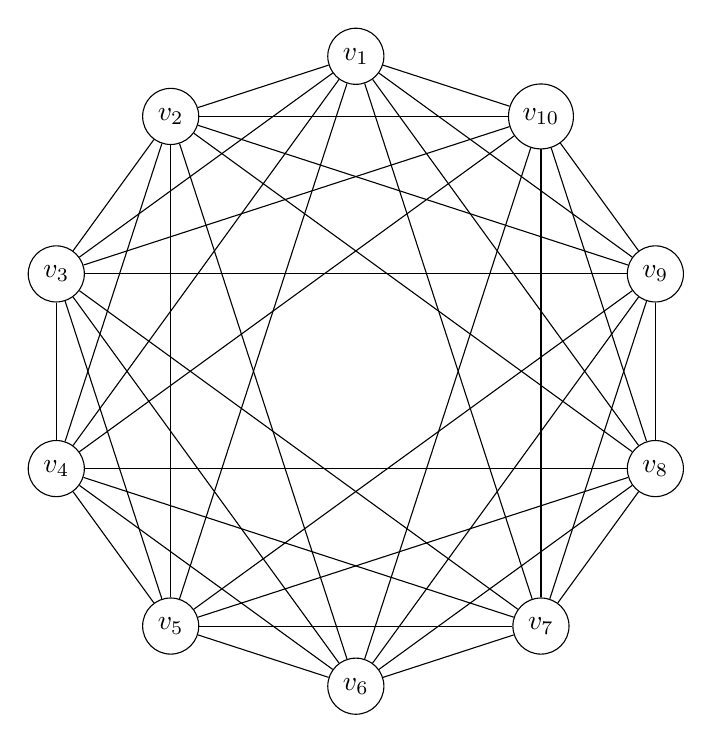
\begin{tikzpicture}
            % 10 vértices de un decágono, con un bucle
            \foreach \x in {1,...,10}
                \node[draw, circle] (v\x) at ({(\x-1)*36+90}:4) {$v_{\x}$};

            % Cada uno de los nodos se conecta con el resto excepto con el +5
            \foreach \x in {1,...,10} {
                \foreach \y in {\x,...,10} {
                    \ifnum\x=\y\relax
                        % No hacer nada si x == y
                    \else
                        \ifnum\y=\numexpr\x+5\relax
                            % No hacer nada si y == x + 5
                        \else
                            \draw (v\x) -- (v\y);
                        \fi
                    \fi
                }
            }
        \end{tikzpicture}
        \caption{Situación del Ejercicio~\ref{ej:1.1}.}
        \label{fig:1.1}
    \end{figure}

    Su matriz de adyacencia es:
    \begin{equation*}
        \begin{pmatrix}
            0 & 1 & 1 & 1 & 1 & 0 & 1 & 1 & 1 & 1 \\
            1 & 0 & 1 & 1 & 1 & 1 & 0 & 1 & 1 & 1 \\
            1 & 1 & 0 & 1 & 1 & 1 & 1 & 0 & 1 & 1 \\
            1 & 1 & 1 & 0 & 1 & 1 & 1 & 1 & 0 & 1 \\
            1 & 1 & 1 & 1 & 0 & 1 & 1 & 1 & 1 & 0 \\
            0 & 1 & 1 & 1 & 1 & 0 & 1 & 1 & 1 & 1 \\
            1 & 0 & 1 & 1 & 1 & 1 & 0 & 1 & 1 & 1 \\
            1 & 1 & 0 & 1 & 1 & 1 & 1 & 0 & 1 & 1 \\
            1 & 1 & 1 & 0 & 1 & 1 & 1 & 1 & 0 & 1 \\
            1 & 1 & 1 & 1 & 0 & 1 & 1 & 1 & 1 & 0 \\
        \end{pmatrix}
    \end{equation*}
\end{ejercicio}

\begin{ejercicio}\label{ej:1.2}
    Seis hermanos (Alonso, Bernardo, Carlos, Daniel, Enrique y Fernando) tienen que emparejarse para compartir habitación en el próximo curso escolar. Cada uno de ellos ha elaborado una lista con los nombres de aquellos con los que quiere emparejarse:
    \begin{itemize}
        \item \ul{Lista de Alonso:} Daniel.
        \item \ul{Lista de Bernardo:} Alonso, Enrique.
        \item \ul{Lista de Carlos:} Daniel, Enrique.
        \item \ul{Lista de Daniel:} Carlos.
        \item \ul{Lista de Enrique:} Daniel, Bernardo, Fernando.
        \item \ul{Lista de Fernando:} Alonso, Bernardo.
    \end{itemize}
    Dibuja el grafo dirigido que modela esta situación.\\

    La situación se puede modelar con el grafo de la Figura~\ref{fig:1.2}, donde cada persona viene representada con un vértice con su inicial.
    \begin{figure}
        \centering
        \begin{tikzpicture}
            % 6 vértices de un decágono, con un bucle. Dentro tienen la inicial del nombre
            \foreach \x/\name in {1/A, 2/B, 3/C, 4/D, 5/E, 6/F}
                \node[draw, circle] (\name) at ({(\x-1)*60}:4) {\name};

            \draw[-Stealth] (A) -- (D);
            \draw[-Stealth] (B) -- (A);
            \draw[-Stealth] (B) to [bend right=15] (E);
            \draw[-Stealth] (C) to [bend right=15] (D);
            \draw[-Stealth] (C) -- (E);
            \draw[-Stealth] (D) to [bend right=15] (C);
            \draw[-Stealth] (E) -- (D);
            \draw[-Stealth] (E) to [bend right=15] (B);            
            \draw[-Stealth] (E) -- (F);
            \draw[-Stealth] (F) -- (A);
            \draw[-Stealth] (F) -- (B);
        \end{tikzpicture}
        \caption{Situación del Ejercicio~\ref{ej:1.2}.}
        \label{fig:1.2}
    \end{figure}


\end{ejercicio}
\begin{ejercicio}\label{ej:1.3}
    Expresa en forma matricial los grafos de la Figura~\ref{fig:1.3}.\\
    \begin{figure}
        \centering
        \begin{subfigure}[b]{0.4\textwidth}
            \centering
            \begin{tikzpicture}
                % Nodos con posiciones relativas
                \node[draw, circle] (A) {A};
                \node[draw, circle, below left=of A] (B) {B};
                \node[draw, circle, below right=of A] (C) {C};
                \node[draw, circle, below=of B] (D) {D};
                \node[draw, circle, below=of C] (E) {E};
                
                % Aristas
                \draw (A) -- (B);
                \draw (A) -- (C);
                \draw (B) -- (C);
                \draw (B) -- (D);
                \draw (C) -- (E);
                \draw (D) -- (E);
            \end{tikzpicture}
            \caption{Grafo~\ref{fig:1.3a}.}
            \label{fig:1.3a}
        \end{subfigure}
        \begin{subfigure}[b]{0.4\textwidth}
            \centering
            \begin{tikzpicture}
                % Nodos con posiciones relativas
                \node[draw, circle] (B) {B};
                \node[draw, circle, right=of B] (C) {C};
                \node[draw, circle, below left=of B] (A) {A};
                \node[draw, circle, below right=of C] (D) {D};
                \node[draw, circle, below right=of A] (F) {F};
                \node[draw, circle, right=of F] (E) {E};
                
                % Aristas: A-B-C-D-E-F
                \draw (A) -- (B);
                \draw (B) -- (C);
                \draw (C) -- (D);
                \draw (D) -- (E);
                \draw (E) -- (F);
                \draw (F) -- (A);
                \draw (D) -- (A);
            \end{tikzpicture}
            \caption{Grafo~\ref{fig:1.3b}.}
            \label{fig:1.3b}
        \end{subfigure}
        \caption{Grafos para el ejercicio~\ref{ej:1.3}.}
        \label{fig:1.3}
    \end{figure}

    La matriz de adyacencia del grafo~\ref{fig:1.3a} es:
    \begin{equation*}
        \begin{pmatrix}
            0 & 1 & 1 & 0 & 0 \\
            1 & 0 & 1 & 1 & 0 \\
            1 & 1 & 0 & 0 & 1 \\
            0 & 1 & 0 & 0 & 1 \\
            0 & 0 & 1 & 1 & 0
        \end{pmatrix}
    \end{equation*}

    La matriz de adyacencia del grafo~\ref{fig:1.3b} es:
    \begin{equation*}
        \begin{pmatrix}
            0 & 1 & 0 & 1 & 0 & 1 \\
            1 & 0 & 1 & 0 & 0 & 0 \\
            0 & 1 & 0 & 1 & 0 & 0 \\
            1 & 0 & 1 & 0 & 1 & 0 \\
            0 & 0 & 0 & 1 & 0 & 1 \\
            1 & 0 & 0 & 0 & 1 & 0
        \end{pmatrix}
    \end{equation*}
\end{ejercicio}

\begin{ejercicio}\label{ej:1.4}
    Sea $G$ un grafo completo con cuatro vértices. Construye todos sus subgrafos salvo isomorfismo.\\

    El grafo completo con cuatro vértices es $K_4$, representado en la Figura~\ref{fig:1.4_1}.
    \begin{figure}
        \centering
        \begin{tikzpicture}[node distance=2cm]
            % Nodos con posiciones relativas
            \node[draw, fill=black, circle, minimum size=0.2cm] (A) {};
            \node[draw, fill=black, circle, minimum size=0.2cm, right=of A] (B) {};
            \node[draw, fill=black, circle, minimum size=0.2cm, below=of A] (C) {};
            \node[draw, fill=black, circle, minimum size=0.2cm, below=of B] (D) {};
            
            % Aristas
            \draw (A) -- (B);
            \draw (A) -- (C);
            \draw (A) -- (D);
            \draw (B) -- (D);
            \draw (C) -- (D);
            \draw (C) -- (B);
        \end{tikzpicture}
        \caption{Grafo $K_4$.}
        \label{fig:1.4_1}
    \end{figure}
    
    
    Para evitar pérdida de subgrafos, sabiendo que $K_4$ tiene $4$ vértices, se pueden construir los siguientes subgrafos:
    \begin{itemize}
        \item No consideramos los subgrafos con 0 vértices.
        \item Tan solo hay un subgrafo con un vértice.
        \item Los subgrafos con dos vértices se encuentran en la Figura~\ref{fig:1.4_2}.
        \item Los subgrafos con tres vértices se encuentran en la Figura~\ref{fig:1.4_3}.
        \item Los subgrafos con cuatro vértices se encuentran en la Figura~\ref{fig:1.4_4}.
    \end{itemize}
    \begin{figure}
        \centering
        \begin{subfigure}[b]{0.5\textwidth}
            \centering
            
\begin{tikzpicture}
                \node[draw, fill=black, circle, minimum size=0.2cm] (A) {};
                \node[draw, fill=black, circle, minimum size=0.2cm, right of=A] (B) {};
            \end{tikzpicture}
            \caption{$|E|=0$.}
        \end{subfigure}\hfill
        \begin{subfigure}[b]{0.5\textwidth}
            \centering
            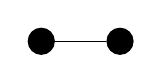
\begin{tikzpicture}
                \node[draw, fill=black, circle, minimum size=0.2cm] (A) {};
                \node[draw, fill=black, circle, minimum size=0.2cm, right of=A] (B) {};

                \draw (A) -- (B);
            \end{tikzpicture}
            \caption{$|E|=1$.}
        \end{subfigure}
        \caption{Subgrafos de $K_4$ con 2 vértices, $|V|=2$.}
        \label{fig:1.4_2}
    \end{figure}
    \begin{figure}
        \centering
        \begin{subfigure}[b]{0.2\textwidth}
            \centering
            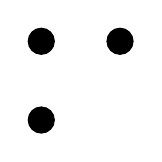
\begin{tikzpicture}
                \node[draw, fill=black, circle, minimum size=0.2cm] (A) {};
                \node[draw, fill=black, circle, minimum size=0.2cm, right of=A] (B) {};
                \node[draw, fill=black, circle, minimum size=0.2cm, below of=A] (C) {};
            \end{tikzpicture}
            \caption{$|E|=0$.}
        \end{subfigure}
        \begin{subfigure}[b]{0.2\textwidth}
            \centering
            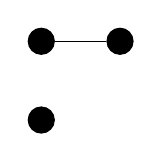
\begin{tikzpicture}
                \node[draw, fill=black, circle, minimum size=0.2cm] (A) {};
                \node[draw, fill=black, circle, minimum size=0.2cm, right of=A] (B) {};
                \node[draw, fill=black, circle, minimum size=0.2cm, below of=A] (C) {};

                \draw (A) -- (B);
            \end{tikzpicture}
            \caption{$|E|=1$.}
        \end{subfigure}
        \begin{subfigure}[b]{0.2\textwidth}
            \centering
            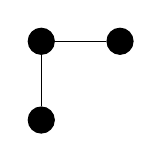
\begin{tikzpicture}
                \node[draw, fill=black, circle, minimum size=0.2cm] (A) {};
                \node[draw, fill=black, circle, minimum size=0.2cm, right of=A] (B) {};
                \node[draw, fill=black, circle, minimum size=0.2cm, below of=A] (C) {};

                \draw (A) -- (B);
                \draw (A) -- (C);
            \end{tikzpicture}
            \caption{$|E|=2$.}
        \end{subfigure}
        \begin{subfigure}[b]{0.2\textwidth}
            \centering
            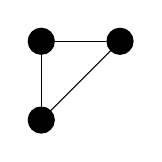
\begin{tikzpicture}
                \node[draw, fill=black, circle, minimum size=0.2cm] (A) {};
                \node[draw, fill=black, circle, minimum size=0.2cm, right of=A] (B) {};
                \node[draw, fill=black, circle, minimum size=0.2cm, below of=A] (C) {};

                \draw (A) -- (B);
                \draw (A) -- (C);
                \draw (B) -- (C);
            \end{tikzpicture}
            \caption{$|E|=3$.}
        \end{subfigure}
        \caption{Subgrafos de $K_4$ con 3 vértices, $|V|=3$.}
        \label{fig:1.4_3}
    \end{figure}
    \begin{figure}
        \centering
        \begin{subfigure}[b]{0.2\textwidth}
            \centering
            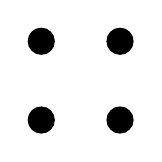
\begin{tikzpicture}
                \node[draw, fill=black, circle, minimum size=0.2cm] (A) {};
                \node[draw, fill=black, circle, minimum size=0.2cm, right of=A] (B) {};
                \node[draw, fill=black, circle, minimum size=0.2cm, below of=A] (C) {};
                \node[draw, fill=black, circle, minimum size=0.2cm, below of=B] (D) {};
            \end{tikzpicture}
            \caption{$|E|=0$.}
        \end{subfigure}
        \begin{subfigure}[b]{0.2\textwidth}
            \centering
            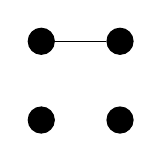
\begin{tikzpicture}
                \node[draw, fill=black, circle, minimum size=0.2cm] (A) {};
                \node[draw, fill=black, circle, minimum size=0.2cm, right of=A] (B) {};
                \node[draw, fill=black, circle, minimum size=0.2cm, below of=A] (C) {};
                \node[draw, fill=black, circle, minimum size=0.2cm, below of=B] (D) {};

                \draw (A) -- (B);
            \end{tikzpicture}
            \caption{$|E|=1$.}
        \end{subfigure}
        \begin{subfigure}[b]{0.2\textwidth}
            \centering
            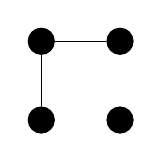
\begin{tikzpicture}
                \node[draw, fill=black, circle, minimum size=0.2cm] (A) {};
                \node[draw, fill=black, circle, minimum size=0.2cm, right of=A] (B) {};
                \node[draw, fill=black, circle, minimum size=0.2cm, below of=A] (C) {};
                \node[draw, fill=black, circle, minimum size=0.2cm, below of=B] (D) {};

                \draw (A) -- (B);
                \draw (A) -- (C);
            \end{tikzpicture}
            \caption{$|E|=2$.}
        \end{subfigure}
        \begin{subfigure}[b]{0.2\textwidth}
            \centering
            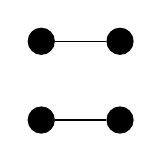
\begin{tikzpicture}
                \node[draw, fill=black, circle, minimum size=0.2cm] (A) {};
                \node[draw, fill=black, circle, minimum size=0.2cm, right of=A] (B) {};
                \node[draw, fill=black, circle, minimum size=0.2cm, below of=A] (C) {};
                \node[draw, fill=black, circle, minimum size=0.2cm, below of=B] (D) {};

                \draw (A) -- (B);
                \draw (C) -- (D);
            \end{tikzpicture}
            \caption{$|E|=2$.}
        \end{subfigure}
        \begin{subfigure}[b]{0.2\textwidth}
            \centering
            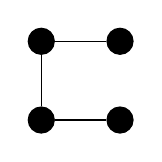
\begin{tikzpicture}
                \node[draw, fill=black, circle, minimum size=0.2cm] (A) {};
                \node[draw, fill=black, circle, minimum size=0.2cm, right of=A] (B) {};
                \node[draw, fill=black, circle, minimum size=0.2cm, below of=A] (C) {};
                \node[draw, fill=black, circle, minimum size=0.2cm, below of=B] (D) {};

                \draw (A) -- (B);
                \draw (A) -- (C);
                \draw (C) -- (D);
            \end{tikzpicture}
            \caption{$|E|=3$.}
        \end{subfigure}
        \begin{subfigure}[b]{0.2\textwidth}
            \centering
            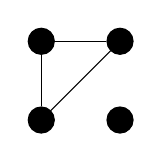
\begin{tikzpicture}
                \node[draw, fill=black, circle, minimum size=0.2cm] (A) {};
                \node[draw, fill=black, circle, minimum size=0.2cm, right of=A] (B) {};
                \node[draw, fill=black, circle, minimum size=0.2cm, below of=A] (C) {};
                \node[draw, fill=black, circle, minimum size=0.2cm, below of=B] (D) {};

                \draw (A) -- (B);
                \draw (A) -- (C);
                \draw (B) -- (C);
            \end{tikzpicture}
            \caption{$|E|=3$.}
        \end{subfigure}
        \begin{subfigure}[b]{0.2\textwidth}
            \centering
            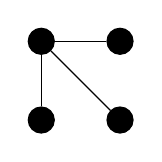
\begin{tikzpicture}
                \node[draw, fill=black, circle, minimum size=0.2cm] (A) {};
                \node[draw, fill=black, circle, minimum size=0.2cm, right of=A] (B) {};
                \node[draw, fill=black, circle, minimum size=0.2cm, below of=A] (C) {};
                \node[draw, fill=black, circle, minimum size=0.2cm, below of=B] (D) {};

                \draw (A) -- (B);
                \draw (A) -- (C);
                \draw (A) -- (D);
            \end{tikzpicture}
            \caption{$|E|=4$.}
        \end{subfigure}
        \begin{subfigure}[b]{0.2\textwidth}
            \centering
            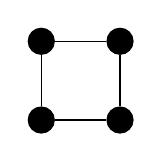
\begin{tikzpicture}
                \node[draw, fill=black, circle, minimum size=0.2cm] (A) {};
                \node[draw, fill=black, circle, minimum size=0.2cm, right of=A] (B) {};
                \node[draw, fill=black, circle, minimum size=0.2cm, below of=A] (C) {};
                \node[draw, fill=black, circle, minimum size=0.2cm, below of=B] (D) {};

                \draw (A) -- (B);
                \draw (A) -- (C);
                \draw (C) -- (D);
                \draw (B) -- (D);
            \end{tikzpicture}
            \caption{$|E|=4$.}
        \end{subfigure}
        \begin{subfigure}[b]{0.2\textwidth}
            \centering
            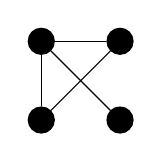
\begin{tikzpicture}
                \node[draw, fill=black, circle, minimum size=0.2cm] (A) {};
                \node[draw, fill=black, circle, minimum size=0.2cm, right of=A] (B) {};
                \node[draw, fill=black, circle, minimum size=0.2cm, below of=A] (C) {};
                \node[draw, fill=black, circle, minimum size=0.2cm, below of=B] (D) {};

                \draw (A) -- (B);
                \draw (A) -- (C);
                \draw (B) -- (C);
                \draw (A) -- (D);
            \end{tikzpicture}
            \caption{$|E|=4$.}
        \end{subfigure}
        \begin{subfigure}[b]{0.2\textwidth}
            \centering
            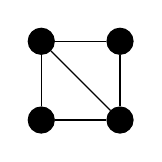
\begin{tikzpicture}
                \node[draw, fill=black, circle, minimum size=0.2cm] (A) {};
                \node[draw, fill=black, circle, minimum size=0.2cm, right of=A] (B) {};
                \node[draw, fill=black, circle, minimum size=0.2cm, below of=A] (C) {};
                \node[draw, fill=black, circle, minimum size=0.2cm, below of=B] (D) {};

                \draw (A) -- (B);
                \draw (A) -- (C);
                \draw (C) -- (D);
                \draw (B) -- (D);
                \draw (A) -- (D);
            \end{tikzpicture}
            \caption{$|E|=5$.}
        \end{subfigure}
        \begin{subfigure}[b]{0.2\textwidth}
            \centering
            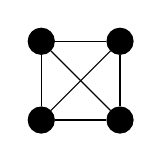
\begin{tikzpicture}
                \node[draw, fill=black, circle, minimum size=0.2cm] (A) {};
                \node[draw, fill=black, circle, minimum size=0.2cm, right of=A] (B) {};
                \node[draw, fill=black, circle, minimum size=0.2cm, below of=A] (C) {};
                \node[draw, fill=black, circle, minimum size=0.2cm, below of=B] (D) {};

                \draw (A) -- (B);
                \draw (A) -- (C);
                \draw (B) -- (C);
                \draw (B) -- (D);
                \draw (A) -- (D);
                \draw (C) -- (D);
            \end{tikzpicture}
            \caption{$|E|=6$.}
        \end{subfigure}
        \caption{Subgrafos de $K_4$ con 4 vértices, $|V|=4$.}
        \label{fig:1.4_4}
    \end{figure}

\end{ejercicio}

\begin{ejercicio}\label{ej:1.5}
    ¿Son isomorfos los grafos de la Figura~\ref{fig:1.5_1}? ¿Y los de la Figura~\ref{fig:1.5_2}? ¿Y los de la Figura~\ref{fig:1.5_3}?\\
    
    \begin{figure}
        \centering
        \begin{subfigure}[b]{0.4\textwidth}
            \centering
            \begin{tikzpicture}
                % Nodos con posiciones relativas
                \node[draw, circle] (A) {A};
                \node[draw, circle, right=of A] (B) {B};
                \node[draw, circle, below=of B] (C) {C};
                \node[draw, circle, below=of A] (D) {D};
                
                % Aristas
                \draw (A) -- (B);
                \draw (A) -- (C);
                \draw (A) -- (D);
                \draw (C) -- (D);
                \draw (C) -- (B);
            \end{tikzpicture}
            \caption{Grafo~\ref{fig:1.5_1.a}.}
            \label{fig:1.5_1.a}
        \end{subfigure}
        \begin{subfigure}[b]{0.4\textwidth}
            \centering
            \begin{tikzpicture}
                % Nodos con posiciones relativas
                \node[draw, circle] (A) {A};
                \node[draw, circle, right=of A] (B) {B};
                \node[draw, circle, below=of B] (C) {C};
                \node[draw, circle, below=of A] (D) {D};
                
                % Aristas
                \draw (A) -- (B);
                \draw (A) -- (C);
                \draw (A) -- (D);
                \draw (C) -- (D);
                \draw (D) -- (B);
            \end{tikzpicture}
            \caption{Grafo~\ref{fig:1.5_1.b}.}
            \label{fig:1.5_1.b}
        \end{subfigure}
        \caption{Primer par de grafos para el ejercicio~\ref{ej:1.5}.}
        \label{fig:1.5_1}
    \end{figure}

    Veamos que los grafos de la Figura~\ref{fig:1.5_1} son isomorfos. Sea $G(V,E)$ el grafo~\ref{fig:1.5_1.a} y $G'(V',E')$ el grafo~\ref{fig:1.5_1.b}.
    Las biyecciones $h_E:E\to E'$ y $h_V:V\to V'$ vienen dadas por:
    \begin{equation*}
        \begin{array}{rlccc}
            h_V & : & V & \to & V'\\
            &  & A & \mapsto & A\\
            &  & B & \mapsto & B\\
            &  & C & \mapsto & D\\
            &  & D & \mapsto & C\\
            &  & E & \mapsto & E
        \end{array}
    \end{equation*}
    \Func{h_E}{E}{E'}{e=\{u,v\}}{e'=\{h_V(u),h_V(v)\}}


    \begin{figure}
        \centering
        \begin{subfigure}[b]{0.4\textwidth}
            \centering
            \begin{tikzpicture}
                % Nodos con posiciones relativas
                \node[draw, circle] (A) {A};
                \node[draw, circle, below left=of A] (B) {B};
                \node[draw, circle, below right=of A] (E) {E};
                \node[draw, circle, below=of B] (C) {C};
                \node[draw, circle, below=of E] (D) {D};
                
                % Aristas
                \draw (A) -- (B);
                \draw (A) -- (E);
                \draw (B) -- (C);
                \draw (B) -- (D);
                \draw (B) -- (E);
                \draw (C) -- (E);
                \draw (C) -- (D);
                \draw (D) -- (E);
            \end{tikzpicture}
            \caption{Grafo~\ref{fig:1.5_2.a}.}
            \label{fig:1.5_2.a}
        \end{subfigure}
        \begin{subfigure}[b]{0.4\textwidth}
            \centering
            \begin{tikzpicture}
                % Nodos con posiciones relativas
                \node[draw, circle] (A) {A};
                \node[draw, circle, below left=of A] (B) {B};
                \node[draw, circle, below right=of A] (E) {E};
                \node[draw, circle, below=of B] (C) {C};
                \node[draw, circle, below=of E] (D) {D};
                
                % Aristas
                \draw (A) -- (B);
                \draw (A) -- (E);
                \draw (B) -- (C);
                \draw (A) -- (D);
                \draw (B) -- (E);
                \draw (C) -- (A);
                \draw (C) -- (D);
                \draw (D) -- (E);
            \end{tikzpicture}
            \caption{Grafo~\ref{fig:1.5_2.b}.}
            \label{fig:1.5_2.b}
        \end{subfigure}
        \caption{Segundo par de grafos para el ejercicio~\ref{ej:1.5}.}
        \label{fig:1.5_2}
    \end{figure}

    Respecto al par de grafos de la Figura~\ref{fig:1.5_2}, sabemos que no son isomorfos puesto que no tienen la misma sucesión de grafos; pues notando por $G(E,V)$ al grafo~\ref{fig:1.5_2.a} y $G'(E',V')$ al grafo~\ref{fig:1.5_2.b}, se tiene que:
    \begin{equation*}
        D_4(G)=0\neq 1=D_4(G')
    \end{equation*}


    \begin{figure}
        \centering
        \begin{subfigure}[b]{0.4\textwidth}
            \centering
            \begin{tikzpicture}
                % Nodos con posiciones relativas
                \node[draw, circle] (B) {B};
                \node[draw, circle, right=of B] (C) {C};
                \node[draw, circle, below left=of B] (A) {A};
                \node[draw, circle, below right=of C] (D) {D};
                \node[draw, circle, below right=of A] (F) {F};
                \node[draw, circle, right=of F] (E) {E};
                
                % Aristas: A-B-C-D-E-F
                \draw (A) -- (B);
                \draw (B) -- (C);
                \draw (C) -- (D);
                \draw (D) -- (E);
                \draw (E) -- (F);
                \draw (F) -- (A);
                \draw (D) -- (A);
                \draw (B) -- (E);
                \draw (F) -- (C);
            \end{tikzpicture}
            \caption{Grafo~\ref{fig:1.5_3.a}.}
            \label{fig:1.5_3.a}
        \end{subfigure}
        \begin{subfigure}[b]{0.4\textwidth}
            \centering
            \begin{tikzpicture}
                % Nodos con posiciones relativas
                \node[draw, circle] (B) {B};
                \node[draw, circle, right=of B] (C) {C};
                \node[draw, circle, left=of B] (A) {A};
                \node[draw, circle, below =of A, yshift=-3em] (D) {D};
                \node[draw, circle, right =of D] (E) {E};
                \node[draw, circle, right =of E] (F) {F};
                
                
                % Aristas: A-D,E,F
                \draw (A) -- (D);
                \draw (A) -- (E);
                \draw (A) -- (F);
                \draw (B) -- (D);
                \draw (B) -- (E);
                \draw (B) -- (F);
                \draw (C) -- (D);
                \draw (C) -- (E);
                \draw (C) -- (F);
            \end{tikzpicture}
            \caption{Grafo~\ref{fig:1.5_3.b}.}
            \label{fig:1.5_3.b}
        \end{subfigure}
        \caption{Tercer par de grafos para el ejercicio~\ref{ej:1.5}.}
        \label{fig:1.5_3}
    \end{figure}

    Por último, veamos que los grafos de la Figura~\ref{fig:1.5_3} son isomorfos. Sea $G(V,E)$ el grafo~\ref{fig:1.5_3.a} y $G'(V',E')$ el grafo~\ref{fig:1.5_3.b}.
    Las biyecciones $h_E:E\to E'$ y $h_V:V\to V'$ vienen dadas por:
    \begin{equation*}
        \begin{array}{rlccc}
            h_V & : & V & \to & V'\\
            &  & A & \mapsto & A\\
            &  & B & \mapsto & D\\
            &  & C & \mapsto & C\\
            &  & D & \mapsto & B\\
            &  & E & \mapsto & E \\
            &  & F & \mapsto & F
        \end{array}
    \end{equation*}
    \Func{h_E}{E}{E'}{e=\{u,v\}}{e'=\{h_V(u),h_V(v)\}}
\end{ejercicio}

\begin{ejercicio}\label{ej:1.6}
    Demostrar que, en cualquier grafo, el número de vértices de grado impar es par.
    (Así, en un grupo de personas, el número total de personas que estrechan la mano de un número impar de otras personas es siempre par).\\

    Sea el grafo $G(V,E)$ con $V$ el conjunto de vértices y $E$ el conjunto de aristas.    
    Sea $I$ el conjunto de vértices de grado impar:
    \begin{equation*}
        I=\{v\in V\mid \deg(v)\text{ es impar}\}.
    \end{equation*}

    Usamos ahora el Lema de Apretón de Manos, descomponiendo $V$ en dos conjuntos disjuntos, $I$ y su complemento $\ol{I}$:
    \begin{equation*}
        \sum_{v\in V}\deg(v)=\sum_{v\in I}\deg(v)+\sum_{v\notin I}\deg(v) =
        2|E| \Longrightarrow
        \sum_{v\in I}\deg(v) = 2|E| - \sum_{v\notin I}\deg(v).
    \end{equation*}

    Por tanto, como $2|E|$ es par, y la suma y resta de números pares es par, tenemos que:
    \begin{equation*}
        \sum_{v\in I}\deg(v) \text{ es par}
    \end{equation*}

    Por la definición de $I$, sabemos que dicha sumatoria es una suma de números impares cuya suma es par. Por tanto, como la suma de dos números impares es par, y la suma de un número par y un número impar es impar, tenemos que la cantidad de elementos en $I$ ha de ser par.
    \begin{equation*}
        |I| \text{ es par}
    \end{equation*}
\end{ejercicio}

\begin{ejercicio}\label{ej:1.7}
    Demostrar que si cada vértice de un grafo $G$ es de grado 2, cada componente conexa de $G$ es un ciclo.\\

    Fijada una componente conexa del grafo $G$, seleccionamos un vértice suyo fijo, sea este $v_0$. Como $\deg v_0=2$, este tendrá dos vértices adyacentes, por lo que seleccionamos uno de ellos; sea este $v_1$. Como $\deg v_1=2$, entonces también tendrá dos vecinos, pero uno de ellos ya lo hemos visitado $(v_0)$, por lo que seleccionamos el otro vecino; sea este $v_3$.
    
    Repitiendo dicho algoritmo seleccionando vértices que no hayamos seleccionado, eventualmente llegaremos a $v_0$ (ya que en caso contrario $V$ no sería finito). Por tanto, habríamos construido un ciclo. Además, como la elección está fijada y se trata de una componente conexa, habremos recorrido todos los vértices de la componente conexa luego, efectivamente, la componente conexa es un ciclo.
\end{ejercicio}

\begin{ejercicio}\label{ej:1.8}
    Los siguientes hechos se conocen de las personas A, B, C, D, E, F, G:
    \begin{itemize}
        \item A habla inglés.
        \item B habla inglés y español.
        \item C habla inglés, italiano y ruso.
        \item D habla japonés y español.
        \item E habla alemán e italiano.
        \item F habla francés, japonés y ruso.
        \item G habla francés y alemán.
    \end{itemize}
    Demostrar que cada par de personas entre estas siete puede comunicarse (con la ayuda de intérpretes, si es necesario, tomados de los cinco restantes).\\

    Construiremos un grafo, en el que dos personas están conectadas por una arista si hablan el mismo idioma. Dicho grafo es el de la Figura~\ref{fig:1.8}. Como se trata de un grafo conexo, dada una persona $p$, podemos llegar a cualquier otra persona $q$ mediante un camino simple (que representan los intérpretes). Por tanto, cada par de personas puede comunicarse.
    \begin{figure}
        \centering
        \begin{tikzpicture}
            % Nodos con posiciones relativas
            \node[draw, circle] (A) {A};
            \node[draw, circle, right=of A] (B) {B};
            \node[draw, circle, below=of B] (C) {C};
            \node[draw, circle, right=of B] (D) {D};
            \node[draw, circle, right=of C] (E) {E};
            \node[draw, circle, right=of D] (F) {F};
            \node[draw, circle, below=of F] (G) {G};
            
            % Aristas
            \draw (A) -- (B);
            \draw (A) -- (C);
            \draw (B) -- (C);
            \draw (B) -- (D);
            \draw (C) -- (E);
            \draw (C) -- (F);
            \draw (D) -- (F);
            \draw (E) -- (G);
            \draw (F) -- (G);
        \end{tikzpicture}
        \caption{Grafo para el ejercicio~\ref{ej:1.8}.}
        \label{fig:1.8}
    \end{figure}
\end{ejercicio}

\begin{ejercicio}\label{ej:1.9}
    Demuestra que en todo grafo con más de un vértice existen dos vértices con el mismo grado.\\

    Supongamos un grafo $G(V,E)$ con $|V|>1$. Como hay $|V|$ vértices, el grado máximo posible es $|V|-1$ (que representaría que dicho vértice está conectado con todos los demás). Por tanto, los posibles grados son:
    \begin{equation*}
        0,1,2,\ldots,|V|-1.
    \end{equation*}

    No obstante, veamos que no todos son posibles; ya que si hay un vértice de grado 0, entonces no puede haber vértices de grado $|V|-1$ (pues dichos vértices no podrían estar conectados con el vértice de grado 0). Por tanto, hay $|V|$ vértices y el número de grados posibles es menor que $|V|$; por lo que, por el principio del palomar, hay al menos dos vértices con el mismo grado.
\end{ejercicio}

\begin{ejercicio}\label{ej:1.10}
    Prueba que si un grafo $G$ contiene solo dos vértices de grado impar entonces ambos han de encontrarse en la misma componente conexa.\\

    Por reducción al absurdo, supongamos que los dos vértices de grado impar se encuentran en componentes conexas distintas; y consideramos $G'(V',E')$ la componente conexa que contiene a uno de ellos (sin pérdida de generalidad, sea $v_1$) y $G''(V'',E'')$ la componente conexa que contiene al otro (sea $v_2$). Como componentes conexas que son, podemos considerarlos como subgrafos de $G$, por lo que $G'$ (se podría trabajar análogamente con $G''$) cumple el Lema del Apretón de Manos:
    \begin{equation*}
        \sum_{v\in V'}\deg(v) = 2|E'| \Longrightarrow \left(\sum_{\substack{v\in V'\\v\neq v_1}}\deg(v)\right) + \deg(v_1) = 2|E'|
    \end{equation*}

    No obstante, la sumatoria sabemos que es una suma de grados pares (pues todos los vértices de $G'$ son de grado par, salvo $v_1$), por lo que es par; y la suma de un número par y un número impar es impar; por lo que no es posible que su suma valga $2|E'|$ (que es par). Por tanto, por reducción al absurdo, los dos vértices de grado impar han de encontrarse en la misma componente conexa.
\end{ejercicio}

\begin{ejercicio}\label{ej:1.11}
    ¿Existe algún grafo regular de grado 5 con 25 vértices?\\

    No, por el Ejericio~\ref{ej:1.6} (25 es impar).
\end{ejercicio}

\begin{ejercicio}\label{ej:1.12}
    ¿Existe un grafo completo con 595 lados?\\

    En un grafo completo, sabemos que:
    \begin{equation*}
        |E| = \frac{|V|(|V|-1)}{2}.
    \end{equation*}

    Suponiendo que fuese posible, como $|E|=595$, tendríamos que:
    \begin{equation*}
        595 = \frac{|V|(|V|-1)}{2} \Longrightarrow |V|^2 - |V| - 1190 = 0
        \Longrightarrow |V| = \frac{1\pm\sqrt{1+4\cdot 1190}}{2} = \frac{1\pm 69}{2}
        \Longrightarrow |V| = 35
    \end{equation*}

    Por tanto, sí es posible, y este es el grafo $K_{35}$.
\end{ejercicio}

\begin{ejercicio}\label{ej:1.13}
    ¿Existe un grafo con 6 vértices cuyos grados sean 1, 2, 2, 3, 4 y 4 respectivamente?

    Buscamos saber si dicha sucesión es gráfica. Para ello, aplicamos el Algoritmo de Havel-Hakimi:
    \begin{table}[H]
        \centering
        \begin{tabular}{cccccc|l}
            4 & 4 & 3 & 2 & 2 & 1 & Eliminamos el 4 y restamos uno a los 4 términos siguientes\\
              & 3 & 2 & 1 & 1 & 1 & Eliminamos el 3 y restamos uno a los 3 términos siguientes\\
              &   & 1 & 0 & 0 & 1 & Reordenamos los términos\\
              &   & 1 & 1 & 0 & 0 & Eliminamos el 1 y restamos uno al término siguiente\\
              &   &   & 0 & 0 & 0 &
        \end{tabular}
    \end{table}

    Llegados a este punto, como la sucesión $0,0,0$ es gráfica, entonces la sucesión $1,2,2,3,4,4$ también lo es. Reconstruimos para ello el grafo; partiendo de la sucesión $0,0,0$, cuyo grafo es el de la Figura~\ref{fig:1.13_1}.
    \begin{figure}
        \centering
        \begin{tikzpicture}
            % Nodos con posiciones relativas
            \node[draw, fill=black, circle, minimum size=0.2cm] (A) {};
            \node[draw, fill=black, circle, minimum size=0.2cm, right=of A] (B) {};
            \node[draw, fill=black, circle, minimum size=0.2cm, right=of B] (C) {};
            
            % Aristas
        \end{tikzpicture}
        \caption{Grafo con sucesión de grados $0,0,0$.}
        \label{fig:1.13_1}
    \end{figure}

    La siguiente sucesión es $1,1,0,0$, que resultó en la sucesión $\textbf{0},0,0$; por lo que hemos de añadir un vértice de grado $1$ que se conecte con uno de los vértices de grado $0$; obteniendo el grafo de la Figura~\ref{fig:1.13_2}.
    \begin{figure}
        \centering
        \begin{tikzpicture}
            % Nodos con posiciones relativas
            \node[draw, fill=black, circle, minimum size=0.2cm] (A) {};
            \node[draw, fill=black, circle, minimum size=0.2cm, left=of A] (D) {};
            \node[draw, fill=black, circle, minimum size=0.2cm, right=of A] (B) {};
            \node[draw, fill=black, circle, minimum size=0.2cm, right=of B] (C) {};
            
            % Aristas
            \draw (A) -- (D);
        \end{tikzpicture}
        \caption{Grafo con sucesión de grados $1,1,0,0$.}
        \label{fig:1.13_2}
    \end{figure}

    La siguiente sucesión es $3,2,1,1,1$, que resultó en la sucesión $\textbf{1,0,0},1$; por lo que hemos de añadir un vértice de grado $3$ que se conecte con un vértice de grado $1$ y dos de grado $0$; obteniendo el grafo de la Figura~\ref{fig:1.13_3}.
    \begin{figure}
        \centering
        \begin{tikzpicture}
            % Nodos con posiciones relativas
            \node[draw, fill=black, circle, minimum size=0.2cm] (A) {};
            \node[draw, fill=black, circle, minimum size=0.2cm, left=of A] (D) {};
            \node[draw, fill=black, circle, minimum size=0.2cm, right=of A] (E) {};
            \node[draw, fill=black, circle, minimum size=0.2cm, right=of E] (B) {};
            \node[draw, fill=black, circle, minimum size=0.2cm, below=of B] (C) {};
            
            % Aristas
            \draw (D) -- (A);
            \draw (E) -- (A);
            \draw (E) -- (B);
            \draw (E) -- (C);
        \end{tikzpicture}
        \caption{Grafo con sucesión de grados $3,2,1,1,1$.}
        \label{fig:1.13_3}
    \end{figure}

    La siguiente sucesión es $4,4,3,2,2,1$, que resultó en la sucesión $\textbf{3,2,1,1},1$; por lo que hemos de añadir un vértice de grado $4$ que se conecte con un vértice de grado $3$, uno de grado $2$ y dos de grado $1$; obteniendo el grafo de la Figura~\ref{fig:1.13_4}.
    \begin{figure}
        \centering
        \begin{tikzpicture}
            % Nodos con posiciones relativas
            \node[draw, fill=black, circle, minimum size=0.2cm] (A) {};
            \node[draw, fill=black, circle, minimum size=0.2cm, left=of A] (D) {};
            \node[draw, fill=black, circle, minimum size=0.2cm, right=of A] (E) {};
            \node[draw, fill=black, circle, minimum size=0.2cm, below=of E] (F) {};
            \node[draw, fill=black, circle, minimum size=0.2cm, right=of E] (B) {};
            \node[draw, fill=black, circle, minimum size=0.2cm, below=of B] (C) {};
            
            % Aristas
            \draw (D) -- (A);
            \draw (E) -- (A);
            \draw (E) -- (B);
            \draw (E) -- (C);
            \draw (F) -- (E);
            \draw (F) -- (A);
            \draw (F) -- (B);
            \draw (F) -- (C);
        \end{tikzpicture}
        \caption{Grafo con sucesión de grados $4,4,3,2,2,1$.}
        \label{fig:1.13_4}
    \end{figure}
\end{ejercicio}

\begin{ejercicio}\label{ej:1.14}
    En cada uno de los siguientes casos, dibuja un grafo de Euler que verifique las condiciones, o prueba que tal grafo no existe:
    \begin{enumerate}
        \item \label{ej:1.14.1}
        Con un número par de vértices y un número par de lados.
        
        Además de $K_{n,m}$ con $m,n$ pares; el grafo de la Figura~\ref{fig:1.14.1} cumple con las condiciones.
        \begin{figure}
            \centering
            \begin{tikzpicture}
                % Nodos con posiciones relativas
                \node[draw, fill=black, circle, minimum size=0.2cm] (A) {};
                \node[draw, fill=black, circle, minimum size=0.2cm, right=of A] (B) {};
                \node[draw, fill=black, circle, minimum size=0.2cm, below=of A] (D) {};
                \node[draw, fill=black, circle, minimum size=0.2cm, below=of B] (C) {};
                
                % Aristas
                \draw (A) -- (B) -- (C) -- (D) -- (A);
            \end{tikzpicture}
            \caption{Grafo para el Ejercicio~\ref{ej:1.14}.\ref{ej:1.14.1}.}
            \label{fig:1.14.1}
        \end{figure}
        \item \label{ej:1.14.2}
        Con un número par de vértices y un número impar de lados.
        
        El grafo de la Figura~\ref{fig:1.14.2} cumple con las condiciones.
        \begin{figure}
            \centering
            \begin{tikzpicture}
                % Nodos con posiciones relativas
                \node[draw, fill=black, circle, minimum size=0.2cm] (A) {};
                \node[draw, fill=black, circle, minimum size=0.2cm, right=of A] (B) {};
                \node[draw, fill=black, circle, minimum size=0.2cm, below=of A] (D) {};
                \node[draw, fill=black, circle, minimum size=0.2cm, below=of B] (C) {};
                \node[draw, fill=black, circle, minimum size=0.2cm, above right=of B] (E) {};
                \node[draw, fill=black, circle, minimum size=0.2cm, below right=of E] (F) {};
                
                % Aristas
                \draw (A) -- (B) -- (E) -- (F) -- (B) -- (C) -- (D) -- (A);
            \end{tikzpicture}
            \caption{Grafo para el Ejercicio~\ref{ej:1.14}.\ref{ej:1.14.2}.}
            \label{fig:1.14.2}
        \end{figure}
        \item\label{ej:1.14.3}
        Con un número impar de vértices y un número par de lados.
        
        Además de $K_5$, el grafo de la Figura~\ref{fig:1.14.3} cumple con las condiciones.
        \begin{figure}
            \centering
            \begin{tikzpicture}
                % Nodos con posiciones relativas
                \node[draw, fill=black, circle, minimum size=0.2cm] (A) {};
                \node[draw, fill=black, circle, minimum size=0.2cm, above right=of A] (B) {};
                \node[draw, fill=black, circle, minimum size=0.2cm, below right=of B] (C) {};
                \node[draw, fill=black, circle, minimum size=0.2cm, above right=of C] (D) {};
                \node[draw, fill=black, circle, minimum size=0.2cm, below right=of D] (E) {};
                
                % Aristas
                \draw (A) -- (B) -- (C) -- (D) -- (E) -- (C) -- (A);
            \end{tikzpicture}
            \caption{Grafo para el Ejercicio~\ref{ej:1.14}.\ref{ej:1.14.3}.}
            \label{fig:1.14.3}
        \end{figure}
        \item\label{ej:1.14.4}
        Con un número impar de vértices y un número impar de lados.

        Además de $K_3$, el grafo de la Figura~\ref{fig:1.14.4} cumple con las condiciones.
        \begin{figure}
            \centering
            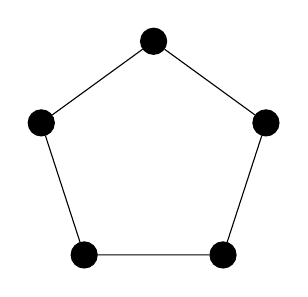
\begin{tikzpicture}
                % Nodos con posiciones relativas
                % Pentangono
                \foreach \i in {0,...,4}
                    \node[draw, fill=black, circle, minimum size=0.2cm, shift=(\i*72+90:1.5)] (\i) {};
                
                % Aristas
                \draw (1) -- (2) -- (3) -- (4) -- (0) -- (1);
            \end{tikzpicture}
            \caption{Grafo para el Ejercicio~\ref{ej:1.14}.\ref{ej:1.14.4}.}
            \label{fig:1.14.4}
        \end{figure}
    \end{enumerate}
\end{ejercicio}

\begin{ejercicio}\label{ej:1.15}
    Encuentra un circuito de Euler para los grafos de la Figura~\ref{fig:1.15}.
    

    \begin{figure}
        \centering
        \begin{subfigure}[b]{0.4\textwidth}
            \centering
            \resizebox{1.2\textwidth}{!}{
            \begin{tikzpicture}[node distance=0.5cm]
                % Nodos con posiciones relativas
                \node[draw, circle] (A) {A};
                \node[draw, circle, below left=of A] (B) {B};
                \node[draw, circle, below right=of A] (C) {C};
                \node[draw, circle, below left=of B] (D) {D};
                \node[draw, circle, below right=of B] (E) {E};
                \node[draw, circle, below right=of C] (F) {F};
                \node[draw, circle, below left=of D] (G) {G};
                \node[draw, circle, below right=of D] (H) {H};
                \node[draw, circle, below left=of F] (I) {I};
                \node[draw, circle, below right=of F] (J) {J};
        
                % Aristas
                \draw (A) -- (B);
                \draw (A) -- (C);
                \draw (B) -- (D);
                \draw (B) -- (C);
                \draw (B) -- (E);
                \draw (C) -- (E);
                \draw (C) -- (F);
                \draw (D) -- (G);
                \draw (D) -- (H);
                \draw (D) -- (E);
                \draw (E) -- (H);
                \draw (E) -- (I);
                \draw (E) -- (F);
                \draw (F) -- (I);
                \draw (F) -- (J);
                \draw (G) -- (H);
                \draw (H) -- (I);
                \draw (I) -- (J);
            \end{tikzpicture}}
            \caption{Grafo~\ref{fig:1.15a}.}
            \label{fig:1.15a}
        \end{subfigure}
        \begin{subfigure}[b]{0.4\textwidth}
            \centering
            \begin{tikzpicture}
                % Nodos con posiciones relativas
                \node[draw, circle] (A) {A};
                \node[draw, circle, below left=of A] (B) {B};
                \node[draw, circle, below right=of A] (C) {C};
                \node[draw, circle, below=of B] (D) {D};
                \node[draw, circle, below=of C] (E) {E};
                \node[draw, circle, below right=of D] (F) {F};
                
                % Aristas
                \draw (A) -- (B);
                \draw (A) -- (C);
                \draw (B) -- (C);
                \draw (B) -- (D);
                \draw (B) -- (E);
                \draw (C) -- (A);
                \draw (C) -- (D);
                \draw (C) -- (E);
                \draw (D) -- (E);
                \draw (D) -- (F);
                \draw (F) -- (E);
            \end{tikzpicture}
            \caption{Grafo~\ref{fig:1.15b}.}
            \label{fig:1.15b}
        \end{subfigure}
        
        \caption{Grafos para el ejercicio~\ref{ej:1.15}.}
        \label{fig:1.15}
    \end{figure}

    Para el grafo de la Figura~\ref{fig:1.15a}, un circuito de Euler es:
    \begin{equation*}
        \hspace{-3em}
        A\to B\to D\to G\to H\to D\to E\to B\to C\to E\to H\to I\to E\to F\to I\to J\to F\to C\to A
    \end{equation*}

    Para el grafo de la Figura~\ref{fig:1.15b}, un circuito de Euler es:
    \begin{equation*}
        B\to A\to C\to B\to E\to C\to D\to F\to E\to D\to B
    \end{equation*}
\end{ejercicio}


\begin{ejercicio}\label{ej:1.16}
    Encuentra un camino de Euler para los grafos de la Figura~\ref{fig:1.16}.
    

    \begin{figure}
        \centering
        \begin{subfigure}[b]{0.4\textwidth}
            \centering
            \begin{tikzpicture}
                % Nodos con posiciones relativas
                \node[draw, circle] (A) {A};
                \node[draw, circle, below left=of A] (C) {C};
                \node[draw, circle, below right=of A] (D) {D};
                \node[draw, circle, below=of C] (F) {F};
                \node[draw, circle, below=of D] (G) {G};
                \node[draw, circle, below right=of F] (I) {I};

                \node[draw, circle, above right=of D] (B) {B};
                \node[draw, circle, below right=of B] (E) {E};
                \node[draw, circle, below=of E] (H) {H};
                \node[draw, circle, below right=of G] (J) {J};
                
                % Aristas
                \draw (A) -- (C);
                \draw (A) -- (D);
                \draw (B) -- (D);
                \draw (B) -- (E);
                \draw (C) -- (D);
                \draw (C) -- (F);
                \draw (C) -- (G);
                \draw (D) -- (E);
                \draw (D) -- (H);
                \draw (D) -- (G);
                \draw (E) -- (H);
                \draw (F) -- (G);
                \draw (F) -- (I);
                \draw (G) -- (J);
                \draw (G) -- (I);
                \draw (H) -- (J);
                \draw (G) -- (H);
                \draw (F) -- (D);
                \draw (G) -- (E);
            \end{tikzpicture}
            \caption{Grafo~\ref{fig:1.16a}.}
            \label{fig:1.16a}
        \end{subfigure}\qquad 
        \begin{subfigure}[b]{0.4\textwidth}
            \centering
            \begin{tikzpicture}
                % Nodos con posiciones relativas
                \node[draw, circle] (A) {A};
                \node[draw, circle, below left=of A] (B) {B};
                \node[draw, circle, below right=of A] (C) {C};
                \node[draw, circle, below=of B] (D) {D};
                \node[draw, circle, below=of C] (E) {E};
                \node[draw, circle, below=of A, yshift=-3.9em] (F) {F};
                \node[draw, circle, below=of D] (G) {G};
                \node[draw, circle, below=of E] (H) {H};
                
                % Aristas
                \draw (A) -- (B);
                \draw (A) -- (C);
                \draw (A) -- (F);
                \draw (B) -- (C);
                \draw (B) -- (D);
                \draw (B) -- (F);
                \draw (C) -- (F);
                \draw (C) -- (E);
                \draw (D) -- (F);
                \draw (E) -- (F);
                \draw (G) -- (F);
                \draw (H) -- (F);
                \draw (G) -- (H);
            \end{tikzpicture}
            \caption{Grafo~\ref{fig:1.16b}.}
            \label{fig:1.16b}
        \end{subfigure}
        
        \caption{Grafos para el ejercicio~\ref{ej:1.16}.}
        \label{fig:1.16}
    \end{figure}

    Para el grafo de la Figura~\ref{fig:1.16a}, un circuito de Euler es:
    \begin{equation*}
        \hspace{-2cm}
        D\to C\to G\to D\to F\to I\to G\to F\to C\to A\to D\to E\to B\to D\to H\to E\to G\to J\to H\to G
    \end{equation*}
    Para el grafo de la Figura~\ref{fig:1.16b}, un circuito de Euler es:
    \begin{equation*}
        A\to B\to C\to A\to F\to D\to B\to F\to C\to E\to F\to G\to H\to F
    \end{equation*}
\end{ejercicio}

\begin{ejercicio}\label{ej:1.17}
    Encontrar un circuito de Euler en el grafo de la Figura~\ref{fig:1.17_1} y un camino de Euler en el grafo de la Figura~\ref{fig:1.17_2}.

    \begin{figure}
        \centering
        \begin{tikzpicture}
            % Nodos con posiciones relativas
            \node[draw, circle] (A) {A};
            \node[draw, circle, right=of A] (B) {B};
            \node[draw, circle, right=of B] (C) {C};
            \node[right=of C] (Ph) {\phantom{C}};
            \node[draw, circle, right=of Ph] (E) {E};
            \node[below=of A] (Ph2) {};
            \node[draw, circle, right=of E] (F) {F};
            \node[draw, circle, below=of Ph2] (G) {G};
            \node[draw, circle, right=of G] (H) {H};
            \node[draw, circle, right=of H] (I) {I};
            \node[draw, circle, below=of Ph] (D) {D};
            \node[draw, circle, right=of I] (J) {J};
            \node[draw, circle, below=of E] (K) {K};
            \node[below=of F] (Ph3) {\phantom{C}};
            \node[draw, circle, below =of Ph3, yshift=-3em] (L) {L};
        
            % Aristas
            \draw (A) -- (B);
            \draw (A) -- (G);
            \draw (B) -- (C);
            \draw (B) -- (G);
            \draw (B) -- (H);
            \draw (B) -- (I);
            \draw (B) -- (J);
            \draw (C) -- (D);
            \draw (C) -- (J);
            \draw (C) -- (E);
            \draw (E) -- (D);
            \draw (E) -- (J);
            \draw (E) -- (F);
            \draw (H) -- (I);
            \draw (I) -- (J);
            \draw (J) -- (L);
            \draw (J) -- (K);
            \draw (K) -- (L);
            \draw (F) -- (L);
            \draw (I) -- (L);
        \end{tikzpicture}
        
        \caption{Primer grafo para el ejercicio~\ref{ej:1.17}.}
        \label{fig:1.17_1}
    \end{figure}

    Para el grafo de la Figura~\ref{fig:1.17_1}, un circuito de Euler es:
    \begin{equation*}
        \hspace{-2cm}
        A\to G\to B\to C\to E\to F\to L\to K\to J\to L\to I\to H\to B\to I\to J\to E\to D\to C\to J\to B\to A
    \end{equation*}


    \begin{figure}
        \centering
        \begin{tikzpicture}
            % Nodos con posiciones relativas
            \node[draw, circle] (A) {A};
            \node[draw, circle, right=of A] (B) {B};
            \node[draw, circle, right=of B] (C) {C};
            \node[draw, circle, right=of C] (D) {D};
            \node[draw, circle, above=of A] (E) {E};
            \node[draw, circle, above=of B] (F) {F};
            \node[draw, circle, above=of C] (G) {G};
            \node[draw, circle, above=of D] (H) {H};
        
            % Aristas
            \draw (A) -- (B);
            \draw (A) -- (F);
            \draw (A) -- (E);
            \draw (B) -- (E);
            \draw (B) -- (F);
            \draw (E) -- (F);
            \draw (B) -- (C);
            \draw (F) -- (G);
            \draw (C) -- (G);
            \draw (C) -- (D);
            \draw (C) -- (H);
            \draw (D) -- (G);
            \draw (G) -- (H);
        \end{tikzpicture}
        
        
        \caption{Segundo grafo para el ejercicio~\ref{ej:1.17}.}
        \label{fig:1.17_2}
    \end{figure}

    Para el grafo de la Figura~\ref{fig:1.17_2}, un camino de Euler es:
    \begin{equation*}
        E\to B\to F\to E\to A\to B \to C\to D\to G\to C\to H\to G\to F\to A
    \end{equation*}
\end{ejercicio}

\begin{ejercicio}\label{ej:1.18}
    ¿Para qué valores de $n$ el grafo $K_n$ es un circuito de Euler?

    El grafo $K_n$ sabemos que es conexo y, al ser completo, todos los vértices tienen grado $n-1$. Además, para que un grafo conexo sea de Euler, todos sus vértices han de tener grado par. Por tanto, $n-1$ ha de ser par, es decir, $n$ ha de ser impar. Por tanto, el grafo $K_n$ es un circuito de Euler si y solo si $n$ es impar.
\end{ejercicio}

\begin{ejercicio}\label{ej:1.19}
    Un viajante vive en la ciudad A y se supone que visita las ciudades B, C y D antes de volver a A. Encontrar la ruta más corta que consuma este viaje si las distancias entre las cuatro ciudades son, en Km:
    \begin{itemize}
        \item 120 entre A y B.
        \item 70 entre B y C.
        \item 140 entre A y C.
        \item 180 entre A y D.
        \item 100 entre B y D.
        \item 110 entre C y D.
    \end{itemize}

    Representamos el problema mediante el grafo de la Figura~\ref{fig:1.19}, que es $K_4$ con las distancias entre las ciudades.
    Para revolver el problema, podríamos usar algoritmos vistos en la Asignatura de Algorítmica, como el algoritmo de Kruskal. No se verá en esta asignatura, puesto que no se considerarán grafos ponderados.
    \begin{figure}
        \centering
        \begin{tikzpicture}[node distance=2cm]
            % Nodos con posiciones relativas
            \node[draw, circle] (A) {A};
            \node[draw, circle, right=of A] (B) {B};
            \node[draw, circle, below=of A] (C) {C};
            \node[draw, circle, below=of B] (D) {D};
        
            % Aristas
            \draw (A) -- node[above]{120} (B);
            \draw (A) -- node[left]{140} (C);
            \draw (A) -- node[above, pos=0.25]{180} (D);
            \draw (B) -- node[above, pos=0.25]{70} (C);
            \draw (B) -- node[right]{100} (D);
            \draw (C) -- node[below]{110} (D);
        \end{tikzpicture}
        
        
        \caption{Grafo para el ejercicio~\ref{ej:1.19}.}
        \label{fig:1.19}
    \end{figure}

\end{ejercicio}

\begin{ejercicio}\label{ej:1.20}
    El grafo línea $L(G)$ de un un grafo $G$ se define como sigue: Los vértices de $L(G)$ son los lados de $G$, $V(L(G)) = E(G)$; y dos vértices en $L(G)$ son adyacentes si y solo si los lados correspondientes en $G$ comparten un vértice. Demostrar:
    \begin{enumerate}
        \item Si $G$ es un grafo conexo regular de grado $r$, entonces $L(G)$ es un grafo de Euler.
        
        Por ser $G$ un grafo conexo, tenemos que todos los vértices están conectados; y por tanto lo están también los lados de $G$. Es decir, dados dos lados cualesquiera de $G$, siempre podemos encontrar una sucesión de vértices adyacentes que los conecten; por lo que $L(G)$ es conexo.
        
        Veamos ahora que el grado de cada vértice de $L(G)$ es par. Dado un vértice $e$ de $L(G)$, este representa un lado de $G$ que conecta dos vértices de $G$, sea $\gamma_G(e)=\{v_1,v_2\}$. Por cada lado de $G$ incidente a $v_1$ o $v_2$ (excepto $e$), hay un vértice adyacente a $e$ en $L(G)$; por lo que:
        \begin{equation*}
            \deg_{L(G)}(e) = \deg_G(v_1) + \deg_G(v_2)-2
        \end{equation*}
        donde se resta $2$ por el lado $e$ que comparten $v_1$ y $v_2$. Por ser $G$ regular de grado $r$, tenemos que:
        \begin{equation*}
            \deg_{L(G)}(e) = r+r-2 = 2r-2=2(r-1)
        \end{equation*}

        Por tanto, como $e$ es un vértice arbitrario de $L(G)$, tenemos de hecho que $L(G)$ es regular de grado $2(r-1)$, es decir, todos los vértices de $L(G)$ tienen grado par. Por tanto, $L(G)$ es un grafo de Euler.
        
        \item Si $G$ es un grafo de Euler entonces $L(G)$ es Hamiltoniano.
        
        Supongamos que $G$ es un grafo de Euler, por lo que podemos encontrar una sucesión de lados $e_1,e_2,\ldots,e_n$ que recorren todos los lados de $G$ una vez sin repetir ninguno. Por la definición de $L(G)$, cada vértice de $L(G)$ representa un lado de $G$; por lo que la sucesión de lados de $G$ se convierte en una sucesión de vértices de $L(G)$ que recorre todos los vértices de $L(G)$ una vez sin repetir ninguno. Además, esto es posible porque dos lados adyacentes en $G$ comparten un vértice, por lo que serán vértices adyacentes en $L(G)$. Por tanto, $L(G)$ es Hamiltoniano.
    \end{enumerate}
\end{ejercicio}

\begin{ejercicio}\label{ej:1.21}
    De entre los grafos de la Figura~\ref{fig:1.21_1} y la Figura~\ref{fig:1.21_2}, ¿cuáles contienen un circuito de Hamilton?
    
    \begin{figure}
        \centering
        \begin{tikzpicture}
            % Nodos con posiciones relativas
            \node[draw, circle] (A) {A};
            \node[draw, circle, below=of A] (C) {C};
            \node[draw, circle, right=of C] (D) {D};
            \node[draw, circle, right=of D] (E) {E};
            \node[draw, circle, above=of E] (B) {B};
            \node[draw, circle, below=of D] (H) {H};
            \node[draw, circle, left=of H] (G) {G};
            \node[draw, circle, left=of G] (F) {F};
            \node[draw, circle, right=of H] (I) {I};
            \node[draw, circle, right=of I] (J) {J};
            \node[draw, circle, below=of F] (L) {L};
            \node[draw, circle, below=of G] (M) {M};
            \node[draw, circle, left=of L] (K) {K};
            \node[draw, circle, below=of I] (N) {N};
            \node[draw, circle, below=of J] (O) {O};
            \node[draw, circle, right=of O] (P) {P};
            \node[draw, circle, below=of L] (Q) {Q};
            \node[draw, circle, right=of Q] (R) {R};
            \node[draw, circle, below=of N, yshift=-0.1em] (S) {S};
            \node[draw, circle, right=of S] (T) {T};
            \node[draw, circle, below right=of R] (U) {U};
            \node[draw, circle, below=of U] (V) {V};


            % Aristas
            \draw (A) -- (B);
            \draw (A) -- (C);
            \draw (C) -- (D);
            \draw (D) -- (E);
            \draw (E) -- (B);
            \draw (D) -- (H);
            \draw (C) -- (F);
            \draw (E) -- (J);
            \draw (F) -- (G);
            \draw (G) -- (H);
            \draw (H) -- (I);
            \draw (I) -- (J);
            \draw (F) -- (L);
            \draw (L) -- (Q);
            \draw (G) -- (M);
            \draw (M) -- (R);
            \draw (I) -- (N);
            \draw (N) -- (S);
            \draw (J) -- (O);
            \draw (O) -- (T);
            \draw (Q) -- (R);
            \draw (R) -- (S);
            \draw (S) -- (T);
            \draw (Q) -- (U);
            \draw (U) -- (T);
            \draw (U) -- (V);
            \draw (K) -- (L);
            \draw (O) -- (P);

            % A-K,   flecha curvada
            \draw (A) to [bend right=35] (K);
            \draw (K) to [bend right=35] (V);
            % B-P,   flecha curvada
            \draw (B) to [bend right=-35] (P);
            \draw (P) to [bend right=-35] (V);
        \end{tikzpicture}
        
        
        \caption{Primer grafo para el ejercicio~\ref{ej:1.21}.}
        \label{fig:1.21_1}
    \end{figure}

    Respecto del grafo de la Figura~\ref{fig:1.21_1}, se comprueba que no cumple ninguna de las condiciones suficientes para ser Hamiltoniano; aunque sí cumple todas las condiciones necesarias. Por tanto, hemos de buscar el circuito de Hamilton a ciegas. Este es:
    \begin{multline*}
        A\to K\to V\to P\to H\to E\to J\to O\to T\to U\to Q\to L\to F\to G\to M\to\\\to R\to S\to N\to I\to H\to D\to C\to A
    \end{multline*}


    \begin{figure}
        \centering
        \begin{tikzpicture}
            % Nodos con posiciones relativas
            \node[draw, circle] (A) {A};
            \node[draw, circle, below=of A] (C) {C};
            \node[draw, circle, below=of C] (E) {E};
            \node[draw, circle, left=of C] (B) {B};
            \node[draw, circle, right=of C] (D) {D};

            % Aristas
            \draw (A) -- (B);
            \draw (A) -- (D);
            \draw (B) -- (C) -- (D) -- (E) -- (B);
        \end{tikzpicture}
        
        
        \caption{Segundo grafo para el ejercicio~\ref{ej:1.21}.}
        \label{fig:1.21_2}
    \end{figure}

    Respecto del grafo de la Figura~\ref{fig:1.21_2}, este no es Hamiltoniano.
\end{ejercicio}

\begin{ejercicio}\label{ej:1.22}~
    \begin{enumerate}
        \item Prueba, utilizando el algoritmo explicado en clase, que la sucesión $4 \geq 4 \geq 4 \geq 3 \geq 3 \geq 3 \geq 2 \geq 1$ es gráfica y, utilizando dicho algoritmo, encuentra un grafo que tenga como sucesión de grados la correspondiente.\\
        
        Aplicamos el Algoritmo de Havel-Hakimi, y posteriormente construimos el grafo correspondiente, que se muestra en la Figura~\ref{fig:1.22}.
        \begin{table}[H]
            \centering
            \begin{tabular}{cccccccc|l}
                4 & 4 & 4 & 3 & 3 & 3 & 2 & 1 & Eliminamos el 4 y restamos uno a los 4 términos siguientes\\
                  & 3 & 3 & 2 & 2 & 3 & 2 & 1 & Reordenamos los términos\\
                  & 3 & 3 & 3 & 2 & 2 & 2 & 1 & Eliminamos el 3 y restamos uno a los 3 términos siguientes\\
                  &   & 2 & 2 & 1 & 2 & 2 & 1 & Reordenamos los términos\\
                  &   & 2 & 2 & 2 & 2 & 1 & 1 & Eliminamos el 2 y restamos uno a los 2 términos siguientes\\
                  &   &   & 1 & 1 & 2 & 1 & 1 & Reordenamos los términos\\
                  &   &   & 2 & 1 & 1 & 1 & 1 & Eliminamos el 2 y restamos uno a los 2 términos siguientes\\
                  &   &   &   & 0 & 0 & 1 & 1 &
            \end{tabular}
        \end{table}

        \begin{figure}
            \centering
            \begin{tikzpicture}
                % Nodos con posiciones relativas
                \node[draw, fill=black, circle, minimum size=0.1cm] (1) {};
                \node[draw, fill=black, circle, minimum size=0.1cm, right=of 1] (7) {};
                \node[draw, fill=black, circle, minimum size=0.1cm, right=of 7] (6) {};
                \node[draw, fill=black, circle, minimum size=0.1cm, below=of 6] (3) {};
                \node[draw, fill=black, circle, minimum size=0.1cm, below=of 7] (8) {};
                \node[draw, fill=black, circle, minimum size=0.1cm, below=of 1] (5) {};
                \node[draw, fill=black, circle, minimum size=0.1cm, below=of 1, yshift=1.7em, xshift=-1.7em] (2) {};
                \node[draw, fill=black, circle, minimum size=0.1cm, below=of 6, yshift=1.7em, xshift=-1.7em] (4) {};

                % Aristas
                \draw (4) -- (3);
                \draw (5) -- (1);
                \draw (5) -- (2);
                \draw (6) -- (3);
                \draw (6) -- (4);
                \draw (7) -- (6);
                \draw (7) -- (5);
                \draw (7) -- (1);
                \draw (8) -- (7);
                \draw (8) -- (5);
                \draw (8) -- (4);
                \draw (8) -- (3);
            \end{tikzpicture}
            \caption{Grafo para el ejercicio~\ref{ej:1.22}.\ref{ej:1.22a}.}
            \label{fig:1.22}
        \end{figure}

                    
        \label{ej:1.22a}
        \item\label{ej:1.22b}
        El grafo con matriz de adyacencia $M$ dada por:
        \[
            M=\begin{pmatrix}
                0 & 1 & 1 & 1 & 0 & 1 & 1 & 0 \\
                1 & 0 & 1 & 1 & 1 & 1 & 1 & 0 \\
                1 & 1 & 0 & 1 & 0 & 1 & 0 & 0 \\
                1 & 1 & 1 & 0 & 0 & 1 & 1 & 1 \\
                0 & 1 & 0 & 0 & 0 & 1 & 1 & 1 \\
                1 & 1 & 1 & 1 & 1 & 0 & 1 & 0 \\
                1 & 1 & 0 & 1 & 1 & 1 & 0 & 1 \\
                0 & 0 & 0 & 1 & 1 & 0 & 1 & 0
            \end{pmatrix}
        \]
        es de Euler o en él hay un camino de Euler entre dos vértices. Razona cuál es la situación y encuentra, en su caso, el circuito o el camino de Euler que existe.\\

        Sabemos que el grado del vértice $v_i$ es la suma de los elementos de la fila $i$ de la matriz de adyacencia. Calculando los grados de los vértices, obtenemos tenemos que todos son pares a excepción de los vértices $v_1$ y $v_8$, por lo que hay un camino de Euler entre ellos. Este lo construimos con el algoritmo de Fleury, obteniendo el camino:
        \begin{multline*}
            v_1\to v_2\to v_3\to v_4\to v_6\to v_7\to v_8\to v_5\to v_2\to v_7\to v_1\to v_6\to \\\to v_3\to v_1\to v_4\to v_7\to v_5\to v_6\to v_2\to v_4\to v_8
        \end{multline*}
    \end{enumerate}
\end{ejercicio}

\begin{ejercicio}\label{ej:1.23}~
    \begin{enumerate}
        \item En el grafo $G$ cuya matriz de adyacencia es
        \[
            M=\begin{pmatrix}
                0 & 1 & 0 & 1 & 1 & 1 & 0 & 0 \\
                1 & 0 & 0 & 0 & 0 & 0 & 0 & 1 \\
                0 & 0 & 0 & 1 & 1 & 1 & 1 & 0 \\
                1 & 0 & 1 & 0 & 0 & 1 & 0 & 1 \\
                1 & 0 & 1 & 0 & 0 & 0 & 0 & 0 \\
                1 & 0 & 1 & 1 & 0 & 0 & 0 & 1 \\
                0 & 0 & 1 & 0 & 0 & 0 & 0 & 1 \\
                0 & 1 & 0 & 1 & 0 & 1 & 1 & 0
            \end{pmatrix}
        \]
        determina el número de aristas y la sucesión de grados de los vértices y, caso de que $G$ sea de Euler, describe un circuito de Euler en él usando el algoritmo apropiado.\\

        Tenemos que:
        \begin{align*}
            \deg v_1 &= 4 & \deg v_2 &= 2 & \deg v_3 &= 4 & \deg v_4 &= 4 \\
            \deg v_5 &= 2 & \deg v_6 &= 4 & \deg v_7 &= 2 & \deg v_8 &= 4
        \end{align*}

        Por tanto, usando el Lema del Apretón de Manos, tenemos que:
        \begin{equation*}
            \sum_{v\in V} \deg v = 4+2+4+4+2+4+2+4 = 26 = 2|E|
            \Longrightarrow |E| = 13
        \end{equation*}

        La sucesión de grados por tanto es:
        \begin{equation*}
            0,0,3,0,5
        \end{equation*}

        Realizando un recorrido del grafo, vemos que el grafo es conexo; y como todos sus vértices tienen grado par, es de Euler. Por tanto, aplicamos el algoritmo de Fleury para encontrar un circuito de Euler, obteniendo el circuito:
        \begin{equation*}
            v_1\to v_2\to v_8\to v_6\to v_1\to v_4\to v_3\to v_6\to v_4\to v_8\to v_7\to v_3\to v_5\to v_1
        \end{equation*}
        
        \item Calcula el número de vértices de un grafo plano, conexo y regular de grado 5 con 20 caras.
        
        Por ser plano y conexo, tenemos que:
        \begin{equation*}
            |V|+20=|E|+2
        \end{equation*}

        Por el Lema del Apretón de Manos, tenemos que:
        \begin{equation*}
            \sum_{v\in V} \deg v = 2|E|\Longrightarrow
            5|V|=2|E|
        \end{equation*}

        Resolvemos por tanto el siguiente sistema:
        \begin{align*}
            |V|+20&=|E|+2\\
            5|V|&=2|E|\Longrightarrow
            |E|=\nicefrac{5}{2}\cdot |V|
        \end{align*}

        Por tanto, tenemos que:
        \begin{equation*}
            |V|+20=\nicefrac{5}{2}\cdot |V|+2
            \Longrightarrow
            |V|=\nicefrac{18\cdot 2}{3}=12
        \end{equation*}
    \end{enumerate}
\end{ejercicio}

\begin{ejercicio}\label{ej:1.24}~
    \begin{enumerate}
        \item\label{ej:1.24a}
        La siguiente matriz es la matriz de incidencia o adyacencia de un grafo. Razona qué caso es y dibuja el correspondiente grafo.
        \[
            M=\begin{pmatrix}
                1 & 0 & 1 & 0 & 0 & 0 & 0 & 0 \\
                1 & 1 & 0 & 0 & 0 & 0 & 0 & 0 \\
                0 & 1 & 0 & 1 & 1 & 0 & 0 & 0 \\
                0 & 0 & 1 & 1 & 0 & 0 & 0 & 0 \\
                0 & 0 & 0 & 0 & 1 & 1 & 1 & 0 \\
                0 & 0 & 0 & 0 & 0 & 1 & 0 & 1 \\
                0 & 0 & 0 & 0 & 0 & 0 & 1 & 1
            \end{pmatrix}
        \]
        ¿Es el grafo anterior de Euler o Hamilton? Razona la respuesta y da un circuito de Euler o Hamilton en caso de que los haya.


        Como no se trata de una matriz cuadrada, no puede ser de adyacencia, por lo que se trata de una matriz de incidencia. El grafo correspondiente es el de la Figura~\ref{fig:1.24_1}.
        \begin{figure}
            \centering
            \begin{tikzpicture}
                % Nodos con posiciones relativas
                \node[draw, circle] (1) {$v_1$};
                \node[draw, circle, below=of 1] (2) {$v_2$};
                \node[draw, circle, right=of 2] (3) {$v_3$};
                \node[draw, circle, right=of 1] (4) {$v_4$};
                \node[draw, circle, right=of 3] (5) {$v_5$};
                \node[draw, circle, right=of 5] (6) {$v_6$};
                \node[draw, circle, above=of 5] (7) {$v_7$};

                % Aristas
                \draw (1) -- node[left]{$e_1$} (2);
                \draw (2) -- node[above]{$e_2$} (3);
                \draw (1) -- node[above]{$e_3$} (4);
                \draw (3) -- node[left]{$e_4$} (4);
                \draw (3) -- node[above]{$e_5$} (5);
                \draw (6) -- node[above]{$e_6$} (5);
                \draw (5) -- node[left]{$e_7$} (7);
                \draw (6) -- node[above]{$e_8$} (7);
            \end{tikzpicture}
            \caption{Grafo para el ejercicio~\ref{ej:1.24}.\ref{ej:1.24a}.}
            \label{fig:1.24_1}
        \end{figure}

        Los grados de los vértices son la suma de las filas de la matriz de incidencia, obteniendo:
        \begin{align*}
            \deg v_1 &= 2 & \deg v_2 &= 2 & \deg v_3 &= 3 & \deg v_4 &= 2 \\
            \deg v_5 &= 3 & \deg v_6 &= 2 & \deg v_7 &= 2
        \end{align*}

        Por tanto, no se trata de un grafo de Euler (pues hay vértices de grado impar), pero sí tiene un camino de Euler entre los vértices $v_3$ y $v_5$, que es:
        \begin{equation*}
            v_3\xRightarrow{e_4}v_4\xRightarrow{e_3}v_1\xRightarrow{e_1}v_2\xRightarrow{e_2}v_3\xRightarrow{e_5}v_5\xRightarrow{e_6}v_6\xRightarrow{e_8}v_7\xRightarrow{e_7}v_5
        \end{equation*}

        Además, no es un grafo de Hamilton, pues contiene una arista puente. Esto implica que no se podrá construir un circuito (aunque no sabemos nada sobre camino) de Hamilton en él.
        
        \item Aplica el algoritmo para comprobar si la siguiente sucesión $$6 \geq 4 \geq 4 \geq 3 \geq 3 \geq 3 \geq 3 \geq 3$$ es, o no es, una sucesión gráfica y, en caso de serlo, también aplica el algoritmo para encontrar un grafo que la tenga como sucesión de grados.\\
        
        No se trata de una sucesión gráfica, pues la suma de los grados es impar, lo que contradice el Lema del Apretón de Manos:
        \begin{equation*}
            \sum_{v\in V} \deg v = 6+4+4+3+3+3+3+3 = 29
        \end{equation*}
    \end{enumerate}
\end{ejercicio}


\begin{ejercicio}\label{ej:1.25}
    Razona cuál es la respuesta correcta en cada una de las siguientes cuestiones (todos los grafos a los que se hace referencia son simples, no tienen lazos ni lados paralelos):
    \begin{enumerate}
        \item El grafo completo $K_n$:
        \begin{enumerate}
            \item Es siempre de Euler.
            \item Es siempre de Hamilton.
            \item Dependiendo de $n$ puede ser, o no, de Hamilton o de Euler.
        \end{enumerate}

        Sabemos que $K_n$ es conexo y que todos sus vértices tienen grado $n-1$. Por tanto, en primer lugar vemos que:
        \begin{equation*}
            K_n\ \text{es de Euler} \iff n\ \text{es impar}
        \end{equation*}

        Por otro lado, sabemos que, para cada par de vértices no adyacentes, se verifica que:
        \begin{equation*}
            \deg v_i + \deg v_j = n-1 + n-1 = 2n-2 \geq n\iff n\geq 2
        \end{equation*}
        Por tanto, sabemos que $K_n$ con $n\geq 2$ es de Hamilton. Además, como $K_1$ y $K_2$ son trivialmente de Hamilton, tenemos que:
        \begin{equation*}
            K_n\ \text{es de Hamilton}~\qquad \forall n\in \mathbb{N}
        \end{equation*}

        Por tanto, la respuesta correcta es la \textbf{b)}.
        \item He encontrado un grafo plano y conexo con 200 vértices y:
        \begin{enumerate}
            \item Un número par de caras y un número impar de lados.
            \item Un número par de lados y un número impar de caras.
            \item Un número par de lados y caras.
        \end{enumerate}

        Por ser plano y conexo, sabemos que:
        \begin{equation*}
            200+|C|=|E|+2
        \end{equation*}
        Por tanto, o bien $|E|$ y $|C|$ son ambos pares, o ambos impares. Por tanto, la respuesta correcta es la \textbf{c)}.
        \item Tengo un grafo con un solo vértice de grado impar $v$:
        \begin{enumerate}
            \item Puedo encontrar un camino que empiece en ese vértice $v$, recorra todos los lados del grafo solo una vez y vuelva a él.
            \item Si añado un lado que conecte ese vértice con otro cualquiera del grafo, pongamos $w$, puedo encontrar un camino que empiece en $v$, recorra todos los lados del grafo (incluido el que he añadido) solo una vez y termine en $w$.
            \item Es imposible tener un grafo como ese.
        \end{enumerate}

        Por el Ejercicio~\ref{ej:1.6}, sabemos que el número de vértices de grado impar en un grafo es par. Por tanto, la respuesta correcta es la \textbf{c)}.
        \item En un grafo plano con cinco componentes conexas y 24 lados:
        \begin{enumerate}
            \item El número de vértices y el número de caras son opuestos módulo 30.
            \item El número de vértices y el número de caras son congruentes módulo 30.
            \item Ninguna de las anteriores es cierta.
        \end{enumerate}

        Por ser plano, tenemos que:
        \begin{equation*}
            |V|+|C|=24+1+5=30
        \end{equation*}

        Por tanto, la respuesta correcta es la \textbf{a)}.
        \item Dado un grafo regular de grado 1, entonces:
        \begin{enumerate}
            \item El grafo no puede ser conexo.
            \item El grafo tiene tantas componentes conexas como vértices.
            \item El grafo tiene tantas componentes conexas como lados.
        \end{enumerate}

        La respuesta correcta es la \textbf{c)}.
        \item Un grafo regular conexo de grado 11 con veinte vértices:
        \begin{enumerate}
            \item Es siempre de Euler.
            \item Es siempre de Hamilton.
            \item Ninguna de las dos respuestas anteriores es cierta.
        \end{enumerate}

        Como es regular de grafo $11$ (impar), sabemos que no es de Euler. Por otro lado, sabemos que, para cada par de vértices no adyacentes, se verifica que:
        \begin{equation*}
            \deg v_i + \deg v_j = 11 + 11 = 22 \geq 20
        \end{equation*}
        Por tanto, sabemos que es de Hamilton. Por tanto, la respuesta correcta es la \textbf{b)}.
        \item Elija la respuesta correcta:
        \begin{enumerate}
            \item Sólo hay dos grafos con cuatro vértices y cuatro lados no isomorfos.
            \item Todos los grafos con cuatro vértices y cuatro lados son isomorfos.
            \item Sólo hay tres grafos con cuatro vértices y cuatro lados no isomorfos.
        \end{enumerate}

        En el Ejercicio~\ref{ej:1.4} vimos que la respuesta correcta es la \textbf{a)}.
        \item Un grafo cuya matriz de adyacencia es
        \[
            \begin{pmatrix}
                0 & 1 & 1 & 0 & 0 & 0 & 0 \\
                1 & 0 & 1 & 0 & 0 & 0 & 0 \\
                1 & 1 & 0 & 0 & 0 & 0 & 0 \\
                0 & 0 & 0 & 0 & 1 & 1 & 0 \\
                0 & 0 & 0 & 0 & 0 & 1 & 1 \\
                0 & 0 & 0 & 1 & 1 & 0 & 0 \\
                0 & 0 & 0 & 1 & 1 & 0 & 0
            \end{pmatrix}
        \]
        \begin{enumerate}
            \item Es de Euler.
            \item No es de Euler pero hay un camino de Euler entre dos vértices.
            \item No es de Euler pero sus componentes conexas sí lo son.
        \end{enumerate}

        No es de Euler, pues no es conexo. Sus componentes conexas, formadas por los vértices $\{v_1,v_2,v_3\}$ y $\{v_4,v_5,v_6,v_7\}$ respectivamente, sí son de Euler por ser conexas y tener todos los grados pares. Por tanto, la respuesta correcta es la \textbf{c)}.
        \item Un grafo cuya matriz de incidencia es
        \[
            \begin{pmatrix}
                1 & 1 & 0 & 0 & 0 \\
                1 & 0 & 1 & 0 & 0 \\
                0 & 1 & 1 & 1 & 1 \\
                0 & 0 & 0 & 1 & 0 \\
                0 & 0 & 0 & 0 & 1
            \end{pmatrix}
        \]
        \begin{enumerate}
            \item Es de Hamilton.
            \item No es de Hamilton pero sus componente conexas sí lo son.
            \item No es de Hamilton y tampoco lo son sus componentes conexas.
        \end{enumerate}

        Este grafo es conexo (el vértice $v_3$ está conectado con todos los demás). Además, como $\deg v_5=1$, sabemos que no es de Hamilton. Por tanto, la respuesta correcta es la \textbf{c)}.
        \item La siguiente matriz
        \[
            A=\begin{pmatrix}
                0 & 1 & 0 & 0 & 0 \\
                1 & 0 & 1 & 0 & 0 \\
                1 & 1 & 0 & 1 & 1 \\
                0 & 0 & 1 & 0 & 1 \\
                0 & 0 & 1 & 1 & 0
            \end{pmatrix}
        \]
        \begin{enumerate}
            \item Puede ser la matriz de adyacencia de un grafo pero no la de incidencia.
            \item Puede ser la matriz de incidencia de un grafo pero no la de adyacencia.
            \item No puede ser la matriz de adyacencia ni la de incidencia de un grafo.
        \end{enumerate}

        Como $a_{13}=0\neq 1=a_{31}$, la matriz no es simétrica y por tanto no puede ser la matriz de adyacencia de un grafo. Por otro lado, como la suma de la tercera columna es $3$, si se tratase de la matriz de incidencia, tendríamos una arista que conecta tres vértices, lo que no es posible en un grafo simple. Por tanto, la respuesta correcta es la \textbf{c)}.
    \end{enumerate}
\end{ejercicio}

\begin{ejercicio}\label{ej:1.26}~
    \begin{enumerate}
        \item\label{ej:1.26a}
        Prueba, utilizando el algoritmo explicado en clase, que la sucesión dada por $3 \geq 3 \geq 2 \geq 2 \geq 2 \geq 2 \geq 2$ es gráfica y, utilizando dicho algoritmo, encuentra un grafo en que los grados de sus vértices sean los términos de esa sucesión. Prueba que el grafo es plano y que satisface el teorema de la característica de Euler.\\
        
        Aplicamos el Algoritmo de Havel-Hakimi, y posteriormente construimos el grafo correspondiente, que se muestra en la Figura~\ref{fig:1.26_a}.
        \begin{table}[H]
            \centering
            \begin{tabular}{ccccccc|l}
                3 & 3 & 2 & 2 & 2 & 2 & 2 & Eliminamos el 3 y restamos uno a los 3 términos siguientes\\
                  & 2 & 1 & 1 & 2 & 2 & 2 & Reordenamos los términos\\
                  & 2 & 2 & 2 & 2 & 1 & 1 & Eliminamos el 2 y restamos uno a los 2 términos siguientes\\
                  &   & 1 & 1 & 2 & 1 & 1 & Reordenamos los términos\\
                  &   & 2 & 1 & 1 & 1 & 1 & Eliminamos el 2 y restamos uno a los 2 términos siguientes\\
                  &   &   & 0 & 0 & 1 & 1 &
            \end{tabular}
        \end{table}

        \begin{figure}
            \centering
            \begin{tikzpicture}
                % Nodos con posiciones relativas
                \node[draw, fill=black, circle, minimum size=0.1cm] (1) {};
                \node[draw, fill=black, circle, minimum size=0.1cm, below=of 1] (2) {};
                \node[draw, fill=black, circle, minimum size=0.1cm, right=of 2] (3) {};
                \node[draw, fill=black, circle, minimum size=0.1cm, right=of 1] (4) {};
                \node[draw, fill=black, circle, minimum size=0.1cm, right=of 3] (5) {};
                \node[draw, fill=black, circle, minimum size=0.1cm, right=of 5] (6) {};
                \node[draw, fill=black, circle, minimum size=0.1cm, above=of 5] (7) {};

                % Aristas
                \draw (1) -- (2);
                \draw (2) -- (3);
                \draw (1) --  (4);
                \draw (3) --  (4);
                \draw (3) -- (5);
                \draw (6) --  (5);
                \draw (5) --  (7);
                \draw (6) --  (7);
            \end{tikzpicture}
            \caption{Grafo para el ejercicio~\ref{ej:1.26}.\ref{ej:1.26a}.}
            \label{fig:1.26_a}
        \end{figure}
        
        \item\label{ej:1.26b}
        Considera los grafos $G_1$ dado por el diagrama de la Figura~\ref{fig:1.26_1} y $G_2$ con matriz de incidencia
        \[
            \begin{pmatrix}
                1 & 1 & 0 & 0 & 0 & 0 & 0 & 1 \\
                1 & 0 & 1 & 1 & 1 & 0 & 0 & 0 \\
                0 & 0 & 0 & 1 & 0 & 1 & 1 & 1 \\
                0 & 1 & 1 & 0 & 0 & 1 & 0 & 0 \\
                0 & 0 & 0 & 0 & 1 & 0 & 1 & 0 \\
            \end{pmatrix}
        \]
        Estudia si son o no isomorfos, si son o no planos, si son o no de Euler o si hay un camino de Euler (en caso afirmativo aplica el algoritmo para calcular un circuito o un camino de Euler) y si son o no de Hamilton (encontrando el camino en caso afirmativo).
        \begin{figure}
            \centering
            \begin{tikzpicture}
                % Nodos con posiciones relativas
                \node[draw, circle] (1) {$1$};
                \node[draw, circle, right=of 1] (2) {$2$};
                \node[draw, circle, below right=of 2] (3) {$3$};
                \node[draw, circle, below left=of 1] (5) {$5$};
                \node[draw, circle, below left=of 3] (4) {$4$};

                % Aristas
                \draw (1) -- (5);
                \draw (1) -- (4);
                \draw (1) -- (3);
                \draw (2) -- (5);
                \draw (2) -- (4);
                \draw (2) -- (3);
                \draw (5) -- (4) -- (3);
            \end{tikzpicture}
            \caption{Grafo $G_1$ para el ejercicio~\ref{ej:1.26}.\ref{ej:1.26b}.}
            \label{fig:1.26_1}
        \end{figure}

        Estudiamos cada aspecto:
        \begin{itemize}
            \item No son isomorfos, puesto que $G_1$ no tiene vértices de grado $2$ y $G_2$ sí ($v_5$).
            \item % // TODO: Grafo Plano
            \item Ninguno de ellos es de Euler, puesto que tienen vértices de grado impar.
            \item $G_1$ no tiene ningún camino de Euler, puesto que hay más de dos vértices de grado impar. $G_1$, no obstante, sí tiene un camino de Euler de $v_1$ a $v_4$:
            \begin{equation*}
                v_1\xRightarrow{e_1}v_2
                \xRightarrow{e_3}v_4
                \xRightarrow{e_2}v_1
                \xRightarrow{e_8}v_3
                \xRightarrow{e_4}v_2
                \xRightarrow{e_5}v_5
                \xRightarrow{e_7}v_3
                \xRightarrow{e_6}v_4
            \end{equation*}
            \item Respecto al circuito de Hamilton, estudiamos en primer lugar $G_1$. Sus grados son:
            \begin{align*}
                \deg v_1 &= 3 & \deg v_2 &= 3 & \deg v_3 &= 3 & \deg v_4 &= 4 & \deg v_5 &= 3
            \end{align*}

            Por tanto, dados dos vértices cualesquiera no adyacentes, se verifica que:
            \begin{equation*}
                \deg v_i + \deg v_j \geq 6\geq 5\Longrightarrow G_1\ \text{es de Hamilton}
            \end{equation*}

            Un posible recorrido de Hamilton para $G_1$ es:
            \begin{equation*}
                1\to 3\to 2\to 5\to 4\to 1
            \end{equation*}

            Por otro lado, estudiamos $G_2$. Sus grados son:
            \begin{align*}
                \deg v_1 &= 3 & \deg v_2 &= 4 & \deg v_3 &= 4 & \deg v_4 &= 3 & \deg v_5 &= 2
            \end{align*}

            Por tanto, dados dos vértices cualesquiera no adyacentes, se verifica que:
            \begin{equation*}
                \deg v_i + \deg v_j \geq 5\geq 5\Longrightarrow G_2\ \text{es de Hamilton}
            \end{equation*}

            Un posible recorrido de Hamilton para $G_2$ es:
            \begin{equation*}
                v_1\xRightarrow{e_1}v_2\xRightarrow{e_5}v_5\xRightarrow{e_7}v_3\xRightarrow{e_6}v_4\xRightarrow{e_2}v_1
            \end{equation*}
        \end{itemize}
    \end{enumerate}
\end{ejercicio}


\begin{ejercicio}\label{ej:1.27}~
    \begin{enumerate}
        \item Si $G$ es un grafo completo con 6 vértices entonces:
        \begin{enumerate}
            \item $G$ es regular de grado 5.
            \item $G$ tiene 20 aristas.
            \item $G$ es de Euler y de Hamilton.
        \end{enumerate}

        Sabemos que $K_6$ es regular de grado $5$ y:
        \begin{equation*}
            |E|=\dfrac{6\cdot 5}{2} = 15
        \end{equation*}

        Además, aunque sí es de Hamilton, no es de Euler, por lo que la respuesta correcta es la \textbf{a)}.
        \item\label{ej:1.27_2}
        Sea $G'$ un subgrafo completo (pleno) de un grafo $G$. Entonces:
        \begin{enumerate}
            \item Si $G$ es de Euler también $G'$ es de Euler.
            \item Si $G$ es de Hamilton también $G'$ es de Hamilton.
            \item Ninguna de las anteriores.
        \end{enumerate}

        \begin{figure}
            \centering
            \begin{subfigure}{0.45\textwidth}
                \centering
                \begin{tikzpicture}
                    % Nodos con posiciones relativas
                    \node[draw, fill=black, circle, minimum size=0.1cm] (1) {};
                    \node[draw, fill=black, circle, minimum size=0.1cm, below=of 1] (2) {};
                    \node[draw, fill=black, circle, minimum size=0.1cm, right=of 2] (3) {};
                    \node[draw, fill=black, circle, minimum size=0.1cm, right=of 1] (4) {};
                    
                    % Aristas
                    \draw (1) -- (2) -- (3) -- (4) -- (1);
                \end{tikzpicture}
                \caption{Grafo $G$.}
                \label{fig:1.27_2_G}
            \end{subfigure}
            \begin{subfigure}{0.45\textwidth}
                \centering
                \begin{tikzpicture}
                    % Nodos con posiciones relativas
                    \node[draw, fill=black, circle, minimum size=0.1cm] (1) {};
                    \node[below=of 1] (2) {};
                    \node[draw, fill=black, circle, minimum size=0.1cm, right=of 2, xshift=0.1em] (3) {};
                \end{tikzpicture}
                \caption{Grafo $G'$.}
                \label{fig:1.27_2_Gp}
            \end{subfigure}
            \caption{Grafos para el ejercicio~\ref{ej:1.27}.\ref{ej:1.27_2}.}
            \label{fig:1.27_2}
        \end{figure}

        Consideramos el contraejemplo de la Figura~\ref{fig:1.27_2}. El grafo $G$ de la Figura~\ref{fig:1.27_2_G} es de Euler y de Hamilton, pero su subgrafo completo $G'$ de la Figura~\ref{fig:1.27_2_Gp} no es ni de Euler ni de Hamilton. Por tanto, la respuesta correcta es la \textbf{c)}.
        \item Seleccione la respuesta correcta:
        \begin{enumerate}
            \item Sólo hay dos grafos con cuatro vértices y 5 lados no isomorfos.
            \item Todos los grafos con cuatro vértices y 5 lados son isomorfos.
            \item Todos los grafos con cuatro vértices y cinco lados son de Euler.
        \end{enumerate}
        En el Ejercicio~\ref{ej:1.4} vimos que la respuesta correcta es la \textbf{b)}.
        \item Sea $G$ un grafo plano conexo regular de grado 6 con 15 caras. Entonces:
        \begin{enumerate}
            \item $G$ tiene 13 vértices.
            \item El número de vértices es el triple del de aristas.
            \item No existe un tal grafo.
        \end{enumerate}
        
        Por ser plano y conexo, sabemos que:
        \begin{equation*}
            |V|+15=|E|+2
        \end{equation*}

        Por ser regular de grado $6$, sabemos que:
        \begin{equation*}
            2|E|=6|V|\Longrightarrow |E|=3|V|
        \end{equation*}

        Por tanto, sustituyendo en la primera ecuación, obtenemos:
        \begin{equation*}
            |V|+15=3|V|+2\Longrightarrow |V|=\frac{13}{2}
        \end{equation*}

        Por tanto, la respuesta correcta es la \textbf{c)}.
        \item Salvo isomorfismos, grafos con 50 vértices y 1225 aristas:
        \begin{enumerate}
            \item Solo hay 1.
            \item Hay 2.
            \item No existen grafos en esas condiciones.
        \end{enumerate}
        Tan solo hay uno, y se trata de $K_{50}$, por lo que la respuesta correcta es la \textbf{a)}.
    \end{enumerate}
\end{ejercicio}


\begin{ejercicio}\label{ej:1.28}~
    \begin{enumerate}
        \item Considera la sucesión $4,4,4,4,4$.
        \begin{enumerate}
            \item Utiliza el algoritmo dado en clase para probar que la sucesión es una sucesión gráfica y para dibujar un grafo $G$ que la tenga como sucesión gráfica.
            \item Calcula las matrices incidencia y adyacencia del grafo $G$ obtenido en el apartado anterior.
            \item ¿Es $G$ de Euler o tiene un camino de Euler? En caso afirmativo, utiliza el algoritmo dado en clase para calcular el circuito o el camino de Euler.
            \item ¿Es $G$ de Hamilton? En caso afirmativo calcula el circuito de Hamilton.
            \item ¿Es $G$ plano? En caso afirmativo comprueba la fórmula de la característica de Euler.
        \end{enumerate}
        \item Demuestra que si $G$ es un grafo de Euler con $n$ vértices que solo tiene 2 vértices de grado 2 entonces el número de aristas es $\geq 2n - 2$.
    \end{enumerate}
\end{ejercicio}

\begin{ejercicio}\label{ej:1.29}~
    \begin{enumerate}
        \item Considera el subconjunto $X = \{(12),(13),(23)\} \subset S_3$ y el siguiente grafo $G$: Los vértices de $G$ son los elementos de $S_3$ y hay un lado entre dos vértices $x$ e $y$ si $xy^{-1} \in X$.
        \begin{enumerate}
            \item Dibuja el grafo.
            \item Calcula sus matrices de incidencia y adyacencia.
            \item ¿Es de Euler o tiene un camino de Euler? En caso afirmativo aplica el algoritmo dado en clase para calcular un ciclo o un camino de Euler.
            \item ¿Es de Hamilton? En caso afirmativo calcula el ciclo de Hamilton.
            \item ¿Es plano? En caso afirmativo comprueba la fórmula de Euler.
        \end{enumerate}
        \item Si $G$ es un grafo con $n$ vértices y $m$ lados. Prueba que $m \leq \frac{n(n-1)}{2}$ y que se da la igualdad si y solo si $G = K_n$ es el grafo completo.
    \end{enumerate}
\end{ejercicio}

\begin{ejercicio}\label{ej:1.30}
    Demuestra, utilizando el algoritmo explicado en clase, que la sucesión de grados de los vértices de un octaedro (poliedro regular con 6 vértices, 8 caras y 12 aristas) es gráfica y, utilizando dicho algoritmo, encuentra un grafo $G$ en que los grados de sus vértices sean los términos de esa sucesión. Encuentra las matrices de adyacencia e incidencia de $G$.
    
    Comprueba que el grafo $G$ es plano y estudia si es de Euler y, en caso afirmativo, determina por algún algoritmo explicado en clase un circuito de Euler para $G$. ¿Es $G$ un grafo de Hamilton? Razona la respuesta.
\end{ejercicio}


\begin{ejercicio}\label{ej:1.31}
    Razona cuál es la respuesta correcta en cada una de las siguientes cuestiones (todos los grafos a los que se hace referencia son simples, no tienen lazos ni lados paralelos):
    \begin{enumerate}
        \item La sucesión $70, 69, 68, \ldots, 3, 2, 1$.
        \begin{enumerate}
            \item Es una sucesión gráfica y su grafo asociado es el completo $K_{70}$.
            \item Es una sucesión gráfica pero su grafo asociado no es $K_{70}$.
            \item No es una sucesión gráfica.
        \end{enumerate}
        \item Tengo un grafo conexo con 6 vértices y 9 lados:
        \begin{enumerate}
            \item Puedo asegurar que es plano.
            \item Puedo asegurar que no es plano.
            \item Puede ser plano o no serlo.
        \end{enumerate}
        \item La sucesión $4, 4, 4, 4$:
        \begin{enumerate}
            \item No es una sucesión gráfica pero si le añadimos al final un 2 si lo es.
            \item No es una sucesión gráfica pero si le añadimos al final un 3 si lo es.
            \item No es una sucesión gráfica pero si le añadimos al final un 4 si lo es.
        \end{enumerate}
        \item Puedo encontrar un grafo plano conexo con:
        \begin{enumerate}
            \item Un número impar de vértices, un número impar de lados y un número impar de caras.
            \item Un número par de vértices, un número par de lados y un número impar de caras.
            \item Un número impar de vértices, un número par de lados y un número impar de caras.
        \end{enumerate}
        \item La sucesión $4, 2, 2, 2, 2$:
        \begin{enumerate}
            \item Es la sucesión de grados de un grafo de Euler y de Hamilton.
            \item Es la sucesión de grados de un grafo de Hamilton y no de Euler.
            \item Es la sucesión de grados de un grafo de Euler y no de Hamilton.
        \end{enumerate}
        \item Un grafo regular de grado 7:
        \begin{enumerate}
            \item Tiene que tener al menos 8 vértices y un número impar de lados.
            \item Tiene que tener al menos 8 vértices pero puede tener un número impar o par de lados.
            \item Lo único que puedo afirmar sobre él es que tiene un número par de vértices.
        \end{enumerate}
    \end{enumerate}
\end{ejercicio}


\begin{ejercicio}\label{ej:1.32}
    Considera el grupo simétrico $S_4$ y el subgrupo suyo $H = \langle (1 2 3) \rangle$.
    \begin{enumerate}
        \item Construye el conjunto cociente $S_4/H$ de clases laterales por la izquierda $xH$.
        \item Para cada clase $xH$ denotamos $m(xH)$ al máximo común divisor de los órdenes de los elementos en $xH$. Considera el grafo $G$ con vértices las clases $xH$ y en el que hay un lado entre $xH$ e $yH$ si $m(xH)$ divide a $m(yH)$ o $m(yH)$ divide a $m(xH)$. Identifica el grafo $G$ dando la sucesión de grados de sus vértices y su matriz de adyacencia. ¿Es $G$ de Euler, de Hamilton o plano?
        \item Considera el subgrafo $G'$ obtenido a partir de $G$ eliminando la clase $1H$, ¿es $G'$ de Euler? En caso afirmativo aplica el algoritmo dado en clase para calcular un circuito de Euler.
    \end{enumerate}
\end{ejercicio}

\begin{ejercicio}\label{ej:1.33}
    Se considera el grupo $Q_2 = \langle x, y \mid x^4 = 1, x^2 = y^2, yx = x^{-1}y \rangle$ y el grafo $G$ cuyos vértices son los elementos de $Q_2$ y en el que, para cualquier $a \in Q_2$, hay un lado entre $a$ y $ax$ y también un lado entre $a$ y $ay$.
    \begin{enumerate}
        \item Comprueba que $G$ es un grafo regular dando la sucesión de grados de sus vértices y calcula su matriz de adyacencia.
        \item Razona si $G$ es un grafo de Hamilton o plano.
        \item Razona si $G$ es un grafo de Euler y, en caso afirmativo, aplica el algoritmo dado en clase para calcular un circuito de Euler.
    \end{enumerate}
\end{ejercicio}

\begin{ejercicio}\label{ej:1.34}
    Se considera el grupo $D_4 = \langle r, s \mid r^4 = 1, s^2 = 1, sr = r^{-1}s \rangle$ y el grafo $G$ cuyos vértices son los elementos de $D_4$ y en el que, para cualquier $a \in D_4$, hay un lado entre $a$ y $ar$ y también un lado entre $a$ y $as$.
    \begin{enumerate}
        \item Comprueba que $G$ es un grafo regular dando la sucesión de grados de sus vértices y calcula su matriz de adyacencia.
        \item Razona si $G$ es un grafo de Hamilton o plano.
        \item Razona si $G$ es un grafo de Euler y, en caso afirmativo, aplica el algoritmo dado en clase para calcular un circuito de Euler.
    \end{enumerate}
\end{ejercicio}


\begin{ejercicio}\label{ej:1.35}
    Se considera el grupo diédrico $D_5 = \langle r, s \mid r^5 = 1, s^2 = 1, sr = r^{-1}s \rangle$ y el grafo $G$ cuyos vértices son los elementos de $D_5$ y en el que, para cualquier $a \in D_5$, hay un lado entre $a$ y $ar$ y también un lado entre $a$ y $as$.
    \begin{enumerate}
        \item Calcula la sucesión de grados de $G$ y razona si $G$ es un grafo de Euler, de Hamilton o plano.
        \item Considera un nuevo grafo $G'$ obtenido añadiendo a $G$ un nuevo vértice adyacente a todos los de $G$. Razona si $G'$ es un grafo de Euler y, en caso afirmativo, aplica algún algoritmo dado en clase para calcular un circuito de Euler.
    \end{enumerate}
\end{ejercicio}

\begin{ejercicio}\label{ej:1.36}
    Razona cuál es la respuesta correcta en cada una de las siguientes cuestiones. Todos los grafos a los que se hace referencia son simples (es decir, no tienen lazos ni lados paralelos).
    \begin{enumerate}
        \item La matriz
        \[
            \begin{pmatrix}
                0 & 1 & 1 & 1 & 1 \\
                1 & 0 & 1 & 1 & 1 \\
                1 & 1 & 0 & 1 & 0 \\
                1 & 1 & 1 & 0 & 1 \\
                1 & 1 & 0 & 1 & 0
            \end{pmatrix}
        \]
        es la de adyacencia de un grafo que:
        \begin{enumerate}
            \item Es de Euler.
            \item No es de Hamilton.
            \item Es plano.
        \end{enumerate}
        \item Un grafo plano conexo regular de grado 8 con 23 caras:
        \begin{enumerate}
            \item No existe.
            \item Tiene 12 aristas.
            \item Tiene 9 vértices.
        \end{enumerate}
        \item Se tiene que:
        \begin{enumerate}
            \item Un grafo que es de Euler y de Hamilton siempre es plano.
            \item Un grafo que es plano y de Euler siempre es de Hamilton.
            \item Ninguna de las respuestas anteriores es cierta.
        \end{enumerate}
        \item Se tiene que:
        \begin{enumerate}
            \item La sucesión $5, 5, 4, 2, 2, 2$ es la sucesión gráfica de un grafo plano.
            \item La sucesión $5, 5, 4, 4, 4, 4$ es la sucesión gráfica de un grafo de Hamilton.
            \item La sucesión $5, 4, 4, 3, 3, 3$ es la sucesión gráfica de un grafo de Euler.
        \end{enumerate}
    \end{enumerate}
\end{ejercicio}

\begin{ejercicio}\label{ej:1.37}
    Considera el grupo simétrico $S_4$ y el subgrupo suyo $H = \langle (1 2 3) \rangle$.
    \begin{enumerate}
        \item Construye el conjunto cociente $\nicefrac{S_4}{\sim_H}$ de clases laterales por la derecha $Hx$, $x \in S_4$.
        \item Para cada clase $Hx$ denotamos $n(Hx)$ al mínimo común múltiplo de los órdenes de los elementos en $Hx$. Considera el grafo $G$ con vértices las clases $Hx$ y en el que hay un lado entre $Hx$ e $Hy$ si $n(Hx)$ divide a $n(Hy)$ o $n(Hy)$ divide a $n(Hx)$. Identifica el grafo $G$ dando la sucesión de grados de sus vértices y su matriz de adyacencia. ¿Es $G$ de Euler, de Hamilton o plano?
        \item Considera, si es posible, un subgrafo $G'$ de $G$ obtenido al suprimir una arista entre dos vértices de $G$ de grado impar. ¿Es $G'$ de Euler? ¿Hay un camino de Euler entre dos vértices de $G'$? En caso afirmativo aplica algún algoritmo dado en clase para calcular un circuito o camino de Euler en $G'$.
    \end{enumerate}
\end{ejercicio}

\begin{ejercicio}\label{ej:1.38}
    Se considera el grupo $A_4$ y su subgrupo $H = \langle (1 2)(3 4) \rangle$. Se considera el grafo $G$ con vértices las clases laterales por la izquierda de $H$ en $A_4$, $xH$, y en el que hay un lado entre $xH$ e $yH$ si $m(xH)$ divide a $m(yH)$ o $m(yH)$ divide a $m(xH)$, donde $m(Hx)$ denota el máximo común divisor de los órdenes de los elementos en $xH$.
    Razone cuál de las siguientes es la respuesta correcta:
    \begin{enumerate}
        \item $G$ es plano pero no es de Hamilton.
        \item $G$ no es plano y tiene dos vértices conectados por un camino de Euler.
        \item $G$ es de Hamilton pero no es de Euler.
    \end{enumerate}
\end{ejercicio}


\begin{ejercicio}\label{ej:1.39}
    Considera el grupo simétrico $S_4$ y el subgrupo suyo $H = \langle (1 2 3 4) \rangle$.
    \begin{enumerate}
        \item Construye el conjunto cociente $S_4/H$ de clases laterales por la izquierda $xH$. ¿Es $H \triangleleft S_4$?
        \item Para cada clase $xH$ denotamos $m(xH)$ al máximo común divisor de los órdenes de los elementos en $xH$. Considera el grafo $G$ con vértices las clases $xH$ y en el que hay un lado entre dos clases $xH$ e $yH$ si $m(xH) = m(yH)$. Identifica el grafo $G$ dando la sucesión de grados de sus vértices y su matriz de adyacencia. ¿Es $G$ de Euler, de Hamilton o plano?
        \item Considera el subgrafo $G'$ obtenido a partir de $G$ eliminando la clase $(1 3)H$. ¿Es $G'$ de Euler? En caso afirmativo aplica algún algoritmo dado en clase para calcular un circuito o camino de Euler en $G'$.
    \end{enumerate}
\end{ejercicio}


\begin{ejercicio}\label{ej:1.40}
    Razona cuál es la respuesta correcta en cada una de las siguientes cuestiones. Todos los grafos a los que se hace referencia son simples (es decir, no tienen lazos ni lados paralelos).
    \begin{enumerate}
        \item Se tiene que:
        \begin{enumerate}
            \item Hay un grafo conexo regular de grado 6 con 22 caras y 24 aristas.
            \item La sucesión $4, 4, 4, 3, 3$ es la sucesión gráfica de un grafo plano que tiene un camino de Euler entre dos vértices.
            \item Un grafo conexo y plano es de Euler si y solo si es de Hamilton.
        \end{enumerate}
        \item La matriz
        \[
            \begin{pmatrix}
                0 & 1 & 1 & 1 & 1 & 1 \\
                1 & 0 & 0 & 0 & 0 & 0 \\
                1 & 0 & 0 & 1 & 1 & 1 \\
                1 & 0 & 1 & 0 & 1 & 1 \\
                1 & 0 & 1 & 1 & 0 & 1 \\
                1 & 0 & 1 & 1 & 1 & 0
            \end{pmatrix}
        \]
        es la de adyacencia de un grafo:
        \begin{enumerate}
            \item Con 11 aristas y que es de Euler y de Hamilton.
            \item Que es conexo y plano pero no de Hamilton.
            \item Que no es de Hamilton ni plano ni de Euler.
        \end{enumerate}
    \end{enumerate}
\end{ejercicio}


\begin{ejercicio}\label{ej:1.41}
    Considera el grupo simétrico $S_4$ y el subgrupo suyo $H = \langle (1 3 4) \rangle$.
    \begin{enumerate}
        \item Construye el conjunto cociente $S_4/\sim_H$ de clases laterales por la derecha $Hx$, $x \in S_4$.
        \item Para cada clase $Hx$ denotamos $n(Hx)$ al mínimo común múltiplo de los órdenes de los elementos en $Hx$. Considera el grafo $G$ con vértices las clases $Hx$ y en el que hay un lado entre $Hx$ y $Hy$ si $n(Hx)$ divide a $n(Hy)$ o $n(Hy)$ divide a $n(Hx)$. Identifica el grafo $G$ dando la sucesión de grados de sus vértices y su matriz de adyacencia.
        \item ¿Hay alguna condición suficiente que asegure que $G$ es de Hamilton? ¿Y necesaria para ser plano? ¿Es $G$ de Euler, de Hamilton o plano?
        \item Considera el subgrafo $G'$ de $G$ obtenido al suprimir la arista entre las clases $H(2 3)$ y $H(2 4)$. ¿Es $G'$ de Hamilton, plano o de Euler? ¿Hay un camino de Euler entre dos vértices de $G'$? En caso afirmativo aplica algún algoritmo dado en clase para calcular un circuito o camino de Euler en $G'$.
    \end{enumerate}
\end{ejercicio}